\documentclass[11pt, a4paper]{article}
%\usepackage{proj1}
\usepackage{natbib}
\usepackage{fancyhdr}  
\usepackage{subcaption}
\usepackage{caption}
\usepackage{graphicx}
\linespread{1.25} 
\setlength{\parindent}{0cm}
\graphicspath{{Images/}}
\usepackage{hyperref}
\usepackage{amsmath}
\usepackage{amsfonts}
\usepackage{amssymb}
\usepackage{amsthm}
\usepackage{mathtools}
\usepackage{commath}
\usepackage{bbm}

%\usepackage[sc,osf]{mathpazo}
\usepackage{subcaption}
\usepackage[a4paper, top=1in, left=1.0in, right=1.0in, bottom=1in, includehead, includefoot]{geometry} %Usually have top as 1in

\usepackage{listings}
\usepackage{color} %red, green, blue, yellow, cyan, magenta, black, white
\definecolor{mygreen}{RGB}{28,172,0} % color values Red, Green, Blue
\definecolor{mylilas}{RGB}{170,55,241}


\hypersetup{colorlinks,linkcolor={black},citecolor={blue},urlcolor={black}}
\usepackage{color}
\urlstyle{same}


\theoremstyle{definition}
\newtheorem{definition}{Definition}[section]

%\newcommand{\Sta}{\rho}
\newcommand{\Adj}{p}
\newcommand{\adj}{q}
%\newcommand{\Con}{u}
\newcommand{\Sta}{\rho}
\newcommand{\Stav}{\mathbf{v}}
\newcommand{\Adja}{\mathbf{p}_\Sigma}
\newcommand{\Adjb}{q}
\newcommand{\Adjc}{\mathbf{p}_{\partial \Sigma}}
\newcommand{\Con}{\mathbf{f}}
\newcommand{\nor}{\mathbf{n}}



\title{End Of Year Report/ Part of Thesis Draft}
\author{Jonna C. Roden\\ \\Supervision by Dr Ben Goddard and Dr John Pearson\\ \\ \vspace{0.5cm} MIGSAA}
\date{\today}


\pagenumbering{gobble}
\begin{document}
	\lstset{language=Matlab,%
		%basicstyle=\color{red},
		breaklines=true,%
		morekeywords={matlab2tikz},
		keywordstyle=\color{blue},%
		morekeywords=[2]{1}, keywordstyle=[2]{\color{black}},
		identifierstyle=\color{black},%
		stringstyle=\color{mylilas},
		commentstyle=\color{mygreen},%
		showstringspaces=false,%without this there will be a symbol in the places where there is a space
		numbers=left,%
		numberstyle={\tiny \color{black}},% size of the numbers
		numbersep=9pt, % this defines how far the numbers are from the text
		emph=[1]{for,end,break},emphstyle=[1]\color{blue}, %some words to emphasise
		%emph=[2]{word1,word2}, emphstyle=[2]{style},    
		basicstyle=\footnotesize\ttfamily,
	}
	
	\maketitle
	\begin{abstract}
		Sum up the below here!
		
	\end{abstract}
	
	\newpage
	\section*{Acknowledgements}
	+Acknowledge People Here+
	\newpage
	\pagenumbering{Roman} 
	\tableofcontents
	%\newpage
	%\listoffigures
	%\listoftables
	\newpage
	\pagenumbering{arabic} % Switch to normal numbers
	%\pagestyle{fancy}
















\section{Introduction}
++ Archer paper has examples for applications - also check extended project and other papers for this ++\\
+++get quotes right, figure out how ;) ++

\section{Literature review on PDE-Constrained Optimization for these PDEs}

While mean-field games were first introduced by Lasry and Lions, \cite{LASRY2006619}, \cite{LASRY2006679},\cite{LASRY4} and \cite{Lasry2007}, and independently by Huang, Caines and Malham\'e,  \cite{Huang1}, under the name Nash certainty equivalence, the optimal control side of this class of problems is quite a new area of research. The main difficulty in the optimal control of mean-field equations is a non-linear, non-local particle interaction term. Therefore, standard results in optimal control theory cannot readily be applied, and new approaches have to be developed to address theoretical and numerical challenges.
\\
\\
There are two types of models that recent work has focussed on. The most popular model is a deterministic microscopic model, which is a generalization of the well-known Cucker-Smale model, see \cite{CuckerSmale1}, \cite{CuckerSmale2}. In the mean-field limit, a Vlasov-type PDE arises. For control problems involving this class of models, the work by Fornasier et al. provides a range of theoretical results on the convergence of the microscopic optimal control problem to a corresponding macroscopic problem, using methods of optimal transport and a $\Gamma$-limit argument, proving existence of optimal controls in the mean-field setting, see \cite{Fornasier_2014},
\cite{Fornasier_2014no2}
and \cite{fornasier_lisini_orrieri_savare_2019}. The work focusses on sparse control strategies, where one or more agents influence a larger crowd.
Additional work on sparse control strategies can be found in \cite{piccoli2014no1}, as well as in the review paper \cite{Fornasier_20161no1}.
In \cite{burger2019meanfield}, an alternative method, an $L_2$ calculus, is developed, and convergence results are proved. The control in this work is applied through the interaction term. 
\\
Numerical advances have been made in \cite{burger2019instantaneous} and \cite{burger2016controlling}, where sparse and other control strategies through the external agents are considered. In both papers a Strang-Splitting scheme, \cite{ChengC.Z1976Tiot}, is applied to solve the optimal control problem. The numerical results verify the convergence of the microscopic control problem to its mean-field limit.
Furthermore, in \cite{albi2016selective}, different selective control strategies are considered, and an iterative numerical method is chosen, where the interaction term is approximated stochastically.
\\
\\
Fewer work has been done on the optimal control of the Fokker-Planck PDE, which arises as the mean-field limit of a stochastic microscopic model. Some theoretical results on this model are published. In \cite{albi2016mean}, the existence of optimal controls for microscopic and macroscopic versions of a class of problems are proved and a rigorous derivation of first-order optimality conditions is given. 
Following this, \cite{carrillo2019mean} discusses the existence and regularity of an optimal control problem of this type on periodic domains, including the well-posedness of the Fokker-Planck equation. In \cite{Pinnau_2017} and  \cite{carrillo2018no1}, the convergence of the microscopic optimal control problem to its mean-field limit is proved.
Numerical results on the model include those presented in \cite{Pinnau_2017}, where a Strang-Splitting scheme, \cite{gilbertstrang1}, is applied, and in which convergence to the mean field optimal control problem is shown numerically. Furthermore, in \cite{albi2016mean}, an optimal control hierarchy, including instantaneous and Boltzmann-type controls, is proposed. The mean-field first-order optimality system in \cite{albi2016mean} is solved using a Chang-Cooper scheme for the forward equation, finite differences for the adjoint equation, while approximating the integrals using a Monte-Carlo scheme. This is coupled by a sweeping algorithm, where updates are made through the gradient equation.
Some numerical results on a porous media version of the Fokker-Planck equation are presented in \cite{carrillo2018no1}. In \cite{Albi_2014no1} and \cite{albi2014kinetic}, steady state solutions to a Fokker-Planck-type PDE are considered, however, the main focus  are Boltzmann-type approaches to solving the optimal control problem.
\\
\\
The most common control types in the literature are flow control, e.g. \cite{albi2016mean}, control through the interaction term, e.g. \cite{Pinnau_2017}, as well as control through external agents, e.g. \cite{Fornasier_2014no2}. 
Most papers do not consider boundary conditions, because it is assumed that the particle distribution is of compact support, see \cite{burger2019meanfield}, \cite{fornasier_lisini_orrieri_savare_2019} or \cite{burger2016controlling}. No-flux boundary conditions, which are of high relevance in applications, are not often found in the literature, but are considered in \cite{albi2016mean} and \cite{carrillo2018no1}.
Our work considers the mean-field equation of Fokker-Planck type, flow-type control or control through a force term and no-flux or Dirichlet boundary conditions, in order to address a broad range of test problems and real world applications. 
\\
\\
As described above, some numerical methods have been developed for solving optimal control problems involving non-local, non-linear PDEs. Most of these papers however focus on other methods and use the mean-field optimal control as verification tool, see \cite{Pinnau_2017}, \cite{albi2016mean}. It takes large computational effort to solve these problems, which increases with dimensionality, see \cite{burger2019instantaneous}, \cite{burger2016controlling}. 
We are proposing a new numerical framework for PDE-constrained optimization applied to multiscale particle dynamics, where a fixed point algorithm is implemented to solve the first-order optimality system. This update scheme is inspired by the sweeping algorithm in \cite{albi2016mean}, and equivalent to the gradient descent method in \cite{Burger1}. The algorithm is coupled with pseudospectral methods, used to discretize space and time domains. This composition of methods offers an efficient and accurate solver for the class of problems discussed. To our knowledge, it is the first time that pseudospectral methods are used in the context of optimal control problems.










\section{Deriving optimality conditions}

\subsection{Standard Problems}
+++ State them here given that the sign is wrong in the old report +++
- derive optimality conditions for all the systems we need \\
- Flow/Force\\
- Neumann / Dirichlet/ Dirichlet non-zero/ Mixed\\
\subsection{Archer Optimality Conditions}
+++ Do a bit of the Archer background here, given that you just read it! ++
- Archer paper optimality conditions (good opportunity to link to some background stuff)

\subsubsection*{PDE-Constrained Optimization Problem}
The domain is $\Sigma=\Omega \times [0,T]$. There are two state variables, the particle density $\Sta$ and the velocity $\Stav$. The control is a force term $\Con$. 
\begin{align*}
&\min_{\Sta,\Stav,\Con } \quad \frac{1}{2}||\Sta - \hat \Sta||_{L_2(\Sigma)}^2 + \frac{\alpha}{2}||\Stav - \hat \Stav||_{L_2(\Sigma)}^2 +\frac{\beta}{2}||\Con||_{L_2(\Sigma)}^2\\
&\text{subject to:}\\
&m \Sta \frac{\partial \Stav}{\partial t} + m \Sta (\Stav \cdot \nabla)\Stav + \Sta \nabla V_{ext} + \nabla \Sta + m\gamma \Sta \Stav +\int_\Omega \rho(r) \rho(r') \nabla V_2(|r-r'|)dr'  +\Con=\mathbf{0} \ \ \ \qquad \ \ \quad\text{in} \quad \Sigma\\
&\frac{\partial \Sta}{\partial t} + \nabla \cdot (\Sta \Stav)=0 \qquad\qquad \qquad\qquad\qquad\quad \quad\quad\qquad \qquad\qquad \qquad\qquad\qquad\quad \qquad\qquad\qquad\quad\ \text{in} \quad \Sigma\\
\\
&\Sta \Stav \cdot \mathbf{n} =0\qquad\qquad \qquad\qquad\qquad\qquad\qquad\qquad\qquad \qquad\qquad \qquad\qquad\qquad \qquad\qquad\qquad\quad \qquad \text{on} \quad \partial  \Sigma\\
& \Sta(r,0)=\Sta_0\\
& \Stav(r,0)=\Stav_0.
\end{align*}
Here, we have:
\begin{align*}
\mathcal{F}[\Sta]=\int_\Omega  \bigg( V_{ext}\Sta + \Sta (\log \Sta -1) +  \int_\Omega \Sta(r) \Sta(r')V_2(|r-r'|)dr' \bigg) dr.
\end{align*}

Then:
\begin{align*}
\rho \nabla \frac{\delta \mathcal{F}[\Sta]}{\delta \Sta} = \Sta \nabla V_{ext} + \nabla \Sta + \int_\Omega \Sta(r) \Sta(r') \nabla V_2(|r-r'|)dr',
\end{align*}
which matches Equation $(29)$ in Archer's paper.
\subsubsection*{The Lagrangian}
The Lagrangian for the above problem is:
\begin{align*}
&\mathcal{L}(\Sta,\Stav,\Con,\Adja,\Adjb,\Adjc) = \int_0^T \int_\Omega  \frac{1}{2}(\Sta - \hat \Sta)^2 drdt +\int_0^T \int_\Omega  \frac{\alpha}{2}(\Stav - \hat \Stav)^2 drdt +\int_0^T \int_\Omega  \frac{\beta}{2}\Con^2 drdt\\
&+ \int_0^T \int_\Omega (m \Sta \frac{\partial \Stav}{\partial t} + m \Sta (\Stav \cdot \nabla)\Stav + \Sta \nabla V_{ext} + \nabla \Sta + m\gamma \Sta \Stav +\int_\Omega \rho(r) \rho(r') \nabla V_2(|r-r'|)dr'+\Con) \cdot \Adja dr dt\\
& + \int_0^T \int_\Omega (\frac{\partial \Sta}{\partial t} + \nabla \cdot (\Sta \Stav)) \Adjb dr dt\\ 
& +\int_0^T \int_{\partial\Omega} \Sta \Stav \cdot \mathbf{n} \Adjc dr dt,
\end{align*}
where $\Adja$, $\Adjb$ and $\Adjc$ are Lagrange multipliers associated with the PDE for $\Stav$, the PDE for $\Sta$ and the boundary condition, respectively.
\subsubsection*{Adjoint Equation 1}

The derivative of $\mathcal{L}$ with respect to $\Sta$ in some direction $h$ is, where ${h} \in C_0^\infty(\Sigma) $:
\begin{align*}
&\mathcal{L}_\Sta(\Sta,\Stav,\Con,\Adja,\Adjb,\Adjc)h = \int_0^T \int_\Omega  (\Sta - \hat \Sta)h drdt \\
&+ \int_0^T \int_\Omega (m h \frac{\partial \Stav}{\partial t}\cdot \Adja + m h( (\Stav \cdot \nabla)\Stav )\cdot \Adja+ h\nabla V_{ext}\cdot \Adja + \nabla h\cdot \Adja)  dr dt\\
&+ \int_0^T \int_\Omega (m\gamma h \Stav +\int_\Omega h(r) \rho(r') \nabla V_2(|r-r'|)dr'+\int_\Omega \rho(r) h(r') \nabla V_2(|r-r'|)dr') \cdot \Adja dr dt\\
& + \int_0^T \int_\Omega (\Adjb\frac{\partial h}{\partial t} + \Adjb\nabla \cdot (h \Stav))  dr dt +\int_0^T \int_{\partial\Omega} \Adjc h\Stav \cdot \mathbf{n}  dr dt,
\end{align*}
where the product rule is used to take the derivative of the interaction term. Looking at different integral terms individually:
\begin{align*}
I_1= \int_0^T \int_\Omega \nabla h\cdot \Adja dr dt = \int_0^T \int_{\partial \Omega} h \Adja \cdot \mathbf{n} dr dt - \int_0^T \int_{\Omega} \nabla\cdot \Adja h dr dt
\end{align*}
 
\begin{align*}
I_2 = \int_0^T \int_\Omega \Adjb\frac{\partial h}{\partial t} dr dt = \int_\Omega h(T) \Adjb(T) dr dt - \int_0^T \int_\Omega  \frac{\partial \Adjb}{\partial t}h dr dt
\end{align*}
Note that ${h}(r,0)=0$, (in order to satisfy the condition for all admissible ${h}$) and so the initial condition vanishes from the above expression.
\begin{align*}
I_3= \int_0^T \int_\Omega \Adjb\nabla \cdot (h \Stav) dr dt = \int_0^T \int_{\partial \Omega} \Adjb \Stav \cdot \mathbf{n} h dr dt - \int_0^T \int_\Omega \nabla \Adjb \cdot \Stav h dr dt.
\end{align*}
Furthermore, we have:
\begin{align*}
I_{2B}&= \int_0^T \int_\Omega \bigg(\int_\Omega \rho(r) h(r') \nabla V_2(|r-r'|)dr'\bigg) \cdot \Adja(r) drdt\\
&=\int_0^T \int_\Omega \int_\Omega \rho(r) h(r') \nabla V_2(|r-r'|) \cdot \Adja(r) drdr'dt,
\end{align*}
swapping the order of integration. Then we have:
\begin{align*}
I_{2B}&= \int_0^T \int_\Omega  h(r')\bigg(\int_\Omega  \rho(r)\nabla V_2(|r-r'|) \cdot \Adja(r) dr \bigg)dr'dt,
\end{align*}
and relabelling $r \to r'$ and $r' \to r$ gives:
\begin{align*}
I_{2B}&= -\int_0^T \int_\Omega  h(r)\bigg(\int_\Omega  \rho(r')\nabla V_2(|r-r'|) \cdot \Adja(r') dr' \bigg)drdt.
\end{align*}
The introduction of the minus sign is due to the relationship $\nabla_r V_2(|r - r'|) = \nabla_{r'} V_2(|r' - r|)$.  (++ Check correct location of comment)+++
Replacing $I_1, I_2, I_{2B}$ and $I_3$ in the derivative gives:
\begin{align*}
&\mathcal{L}_\Sta(\Sta,\Stav,\Con,\Adja,\Adjb,\Adjc)h = \int_\Omega h(T) \Adjb(T) dr dt  \\
&+ \int_0^T \int_\Omega ( (\Sta - \hat \Sta) +m  \frac{\partial \Stav}{\partial t}\cdot \Adja + m  ((\Stav \cdot \nabla)\Stav )\cdot \Adja+ \nabla V_{ext}\cdot \Adja -\nabla\cdot \Adja  - \ \nabla \Adjb \cdot \Stav  -  \frac{\partial \Adjb}{\partial t}) h dr dt \\
&+ \int_0^T \int_\Omega  \bigg(\int_\Omega  \rho(r')(\Adja(r) - \Adja(r')) \cdot\nabla V_2(|r-r'|)   dr' + m \gamma \Stav \cdot \Adja \bigg)hdr dt\\
&+\int_0^T \int_{\partial \Omega} ( \Adja \cdot \mathbf{n}  +  \Adjb \Stav \cdot \mathbf{n}   +\Adjc \Stav \cdot \mathbf{n})h  dr dt
\end{align*}
Setting $\mathcal{L}_\Sta(\Sta,\Stav,\Con,\Adja,\Adjb,\Adjc)h=0$, and restricting the admissible set of choices of $h$ to:
\begin{align*}
h&=0 \quad \text{on} \quad \partial \Sigma\\
h(T)&=0.
\end{align*}
Then the derivative becomes:
\begin{align*}
 &\int_0^T \int_\Omega ( (\Sta - \hat \Sta) +m  \frac{\partial \Stav}{\partial t}\cdot \Adja + m  ((\Stav \cdot \nabla)\Stav )\cdot \Adja+ \nabla V_{ext}\cdot \Adja -\nabla\cdot \Adja  - \ \nabla \Adjb \cdot \Stav  -  \frac{\partial \Adjb}{\partial t}) h dr dt \\
 &+ \int_0^T \int_\Omega \bigg( m \gamma \Stav \cdot \Adja+ \int_\Omega  \rho(r')(\Adja(r) - \Adja(r')) \cdot\nabla V_2(|r-r'|)   dr'  \bigg)hdr dt\\
 &=0.
\end{align*}
Since this has to hold for all $h \in C_0^\infty(\Sigma)$ and $C_0^\infty(\Sigma)$ is dense in $L_2(\Sigma)$, the first adjoint equation is derived as:
\begin{align}
&(\Sta - \hat \Sta) +m  \frac{\partial \Stav}{\partial t}\cdot \Adja + m ( (\Stav \cdot \nabla)\Stav) \cdot \Adja+ \nabla V_{ext}\cdot \Adja -\nabla\cdot \Adja  - \ \nabla \Adjb \cdot \Stav  -  \frac{\partial \Adjb}{\partial t}\\
&+ m \gamma \Stav \cdot \Adja + \int_\Omega  \rho(r')(\Adja(r') + \Adja(r)) \cdot\nabla V_2(|r-r'|)   dr'  =0 \qquad\qquad\qquad\qquad\qquad \text{in} \quad \Sigma .\notag
\end{align}
Then, relaxing the conditions on $h$, such that $h(T) \neq 0$ is a permissible choice, gives:
\begin{align*}
\int_\Omega h(T) \Adjb(T) dr dt=0,
\end{align*}
and by the same density argument as above, this gives the final time condition for $\Adjb$:
\begin{align*}
\Adjb(T) = {0} .
\end{align*}
Finally, allowing $h \neq 0 \quad \text{on} \quad \partial \Sigma$ result in:
\begin{align*}
\int_0^T \int_{\partial \Omega} ( \Adja \cdot \mathbf{n}  +  \Adjb \Stav \cdot \mathbf{n}   +\Adjc \Stav \cdot \mathbf{n})h  dr dt=0,
\end{align*}
and again by a density argument:
\begin{align*}
 \Adja \cdot \mathbf{n}  +  \Adjb \Stav \cdot \mathbf{n}   +\Adjc \Stav \cdot \mathbf{n} = 0\qquad \text{on} \quad \partial \Sigma
\end{align*}
Since $\Stav \cdot \mathbf{n} =0$ on $ \partial \Sigma$, the boundary condition reduces to:
\begin{align*}
\Adja \cdot \mathbf{n} = 0 \qquad \text{on} \quad \partial \Sigma.
\end{align*}
Therefore, the first adjoint equation of this problem is:
\begin{align*}
&(\Sta - \hat \Sta) +m  \frac{\partial \Stav}{\partial t}\cdot \Adja + m ( (\Stav \cdot \nabla)\Stav) \cdot \Adja+ \nabla V_{ext}\cdot \Adja -\nabla\cdot \Adja  - \ \nabla \Adjb \cdot \Stav  -  \frac{\partial \Adjb}{\partial t}\\
&+ m \gamma \Stav \cdot \Adja + \int_\Omega  \rho(r')(\Adja(r) - \Adja(r')) \cdot\nabla V_2(|r-r'|)   dr'  =0 \qquad\qquad\qquad\qquad\qquad \text{in} \quad \Sigma \\
& \Adja \cdot \mathbf{n} = 0 \qquad \text{on} \quad \partial \Sigma\\
 &\Adjb(T) = {0} .
\end{align*}

\subsubsection*{Adjoint Equation 2}
Taking the derivative of the above Lagrangian with respect to $\Stav$ in the direction $\mathbf{h} \in C_0^\infty(\Sigma)$, gives:
\begin{align*}
\mathcal{L}_\Stav(\Sta,\Stav,\Con,\Adja,\Adjb,\Adjc)\mathbf{h} &= \int_0^T \int_\Omega 
 \alpha(\Stav - \hat \Stav)\cdot \mathbf{h} drdt  \\
&+ \int_0^T \int_\Omega (m \Sta \frac{\partial \mathbf{h} }{\partial t} + m \Sta (\mathbf{h} \cdot \nabla)\Stav + m \Sta (\Stav \cdot \nabla)\mathbf{h} + m \gamma \Sta \mathbf{h}) \cdot \Adja dr dt\\
& + \int_0^T \int_\Omega ( \nabla \cdot (\Sta \mathbf{h})) \Adjb dr dt\\ 
& +\int_0^T \int_{\partial\Omega} \Sta \mathbf{h} \cdot \mathbf{n} \Adjc dr dt.
\end{align*}

Some of the terms are considered separately, as in the previous calculations:

\begin{align*}
I_4 &= \int_0^T \int_\Omega m \Sta \frac{\partial \mathbf{h} }{\partial t} \cdot \Adja dr dt \\
&= \int_\Omega m \Sta(T) \Adja(T) \cdot \mathbf{h}(T) dr dt - \int_0^T \int_\Omega  m\frac{\partial \Sta}{\partial t} \Adja \cdot \mathbf{h} dr dt - \int_0^T \int_\Omega m \Sta \frac{\partial \Adja}{\partial t} \cdot \mathbf{h} dr dt.
\end{align*}
Note that $\mathbf{h}(0)=\mathbf{0}$, in order to satisfy the conditions on $\mathbf{h}$, as before.
\begin{align*}
I_5= \int_0^T \int_\Omega \Adjb\nabla \cdot ( \Sta \mathbf{h}) dr dr = \int_0^T \int_{\partial \Omega} \Adjb \Sta  \mathbf{n}\cdot \mathbf{h} dr dt - \int_0^T \int_\Omega \Sta\nabla \Adjb \cdot  \mathbf{h} dr dt
\end{align*}

\begin{align*}
I_6 = \int_0^T \int_\Omega m \Sta ((\mathbf{h} \cdot \nabla)\Stav ) \cdot\Adja dr dt = \int_0^T \int_\Omega m \Sta ((\nabla \Stav)^\top\Adja) \cdot  \mathbf{h} dr dt
\end{align*}

\begin{align*}
I_7&=\int_0^T \int_\Omega m \Sta ((\Stav \cdot \nabla)\mathbf{h}) \cdot \Adja dr dt
= \int_0^T \int_{\partial \Omega} m \Sta (\Stav \cdot \Adja)(\mathbf{n} \cdot \mathbf{h})dr dt \\
&- \int_0^T \int_\Omega (m \Sta ((\Stav \cdot \nabla)\Adja)\cdot \mathbf{h} + m \Sta (\nabla \cdot \Stav)(\Adja \cdot \mathbf{h}) + m (\Stav \cdot \nabla \Sta)(\Adja \cdot \mathbf{h}))drdt
\end{align*}
Replacing the rewritten integrals gives:
\begin{align*}
&\mathcal{L}_\Stav(\Sta,\Stav,\Con,\Adja,\Adjb,\Adjc) \mathbf{h} = \int_\Omega m \Sta(T) \Adja(T) \cdot \mathbf{h}(T) dr dt\\
&+\int_0^T \int_\Omega 
\bigg(\alpha(\Stav - \hat \Stav)   - m \frac{\partial \Sta}{\partial t} \Adja  -  m\Sta \frac{\partial \Adja}{\partial t} +m \gamma \Sta \Adja\\
&-\Sta\nabla \Adjb +m \Sta (\nabla \Stav)^\top\Adja 
-m \Sta (\Stav \cdot \nabla)\Adja - m \Sta (\nabla \cdot \Stav)\Adja  - m (\Stav \cdot \nabla \Sta)\Adja  \bigg)\cdot  \mathbf{h} drdt\\
& +\int_0^T \int_{\partial\Omega} ( m \Sta (\Stav \cdot \Adja)+\Sta  \Adjc + \Adjb \Sta)  \mathbf{n}\cdot \mathbf{h} dr dt\\
\end{align*}
Then, setting $\mathcal{L}_\Stav(\Sta,\Stav,\Con,\Adja,\Adjb,\Adjc) \mathbf{h}=\mathbf{0}$ and placing the restrictions on $\mathbf{h}$, as before:
\begin{align*}
\mathbf{h}&=0 \quad \text{on} \quad \partial \Sigma\\
\mathbf{h}(T)&=0,
\end{align*}
gives:
\begin{align*}
&\int_0^T \int_\Omega 
\bigg(\alpha(\Stav - \hat \Stav)   - m \frac{\partial \Sta}{\partial t} \Adja  -  m\Sta \frac{\partial \Adja}{\partial t} +m \gamma \Sta \Adja\\
&-\Sta\nabla \Adjb +m \Sta (\nabla \Stav)^\top\Adja 
-m \Sta (\Stav \cdot \nabla)\Adja - m \Sta (\nabla \cdot \Stav)\Adja  - m (\Stav \cdot \nabla \Sta)\Adja  \bigg)\cdot  \mathbf{h} drdt=0.
\end{align*}
Employing the density argument that $C_0^\infty(\Sigma)$ is dense in $L_2(\Sigma)$, which has to hold for all $\mathbf{h}\in C_0^\infty(\Sigma)$, results in:
\begin{align*}
&\alpha(\Stav - \hat \Stav)   - m \frac{\partial \Sta}{\partial t} \Adja  -  m\Sta \frac{\partial \Adja}{\partial t} 
-\Sta\nabla \Adjb +m \Sta (\nabla \Stav)^\top \Adja +m \gamma \Sta \Adja \\
&-m \Sta (\Stav \cdot \nabla)\Adja - m \Sta (\nabla \cdot \Stav)\Adja  - m (\Stav \cdot \nabla \Sta)\Adja=\mathbf{0} \ \qquad\qquad \text{in} \quad \Sigma.
\end{align*}
Then, relaxing the conditions on $\mathbf{h}$, so that $\mathbf{h}(T) \neq 0 $ is permissible, gives
\begin{align*}
 \int_\Omega m \Sta(T) \Adja(T) \cdot \mathbf{h}(T) dr dt=0,
\end{align*}
and so, since $\Sta \neq 0$, this results in the final time condition for $\Adja$:
\begin{align}
\Adja(T)=\mathbf{0}.
\end{align}
Finally, relaxing the condition $\mathbf{h}=0 \quad \text{on} \quad \partial \Sigma$ gives:
\begin{align*}
\int_0^T \int_{\partial\Omega} ( m \Sta (\Stav \cdot \Adja)+\Sta  \Adjc + \Adjb \Sta)  \mathbf{n}\cdot \mathbf{h} dr dt=0,
\end{align*}
and by the same density argument as above, this results in:
\begin{align*}
(m \Sta (\Stav \cdot \Adja)+\Sta  \Adjc + \Adjb \Sta) \mathbf{n} =\mathbf{0} \qquad \qquad\qquad\qquad\qquad\qquad \quad \text{on} \quad \partial \Sigma.
\end{align*}
This condition can be rewritten, since $\Sta \neq 0$:
\begin{align*}
&(m (\Stav \cdot \Adja)+  \Adjc + \Adjb) \mathbf{n} =\mathbf{0}
\end{align*}
The vectors $\Stav$ and $\Adja$ can be decomposed in terms of the normal direction $\mathbf{n}$ and all perpendicular directions $\mathbf{n}^\perp$:
\begin{align*}
\Stav &= |\Stav^n|\mathbf{n} + |\Stav^{\perp}| \mathbf{n}^\perp\\
\Adja &= |\Adja^n|\mathbf{n} + |\Adja^{\perp}| \mathbf{n}^\perp.
\end{align*}
Therefore:
\begin{align*}
&m \bigg((|\Stav^n|\mathbf{n} + |\Stav^\perp|\mathbf{n}^\perp) \cdot (|\Adja^n|\mathbf{n} + |\Adja^\perp|\mathbf{n}^\perp)\bigg)\mathbf{n}+  \Adjc\mathbf{n} + \Adjb \mathbf{n} =\mathbf{0}.
\end{align*}
Then:
\begin{align*}
&m \bigg((|\Stav^n||\Adja^n|\mathbf{n} \cdot \mathbf{n} + |\Stav^\perp||\Adja^n|\mathbf{n}^\perp \cdot \mathbf{n} + |\Stav^n||\Adja^\perp|\mathbf{n} \cdot\mathbf{n}^\perp+|\Stav^\perp||\Adja^\perp|\mathbf{n}^\perp \cdot \mathbf{n}^\perp)\bigg)\mathbf{n}+  \Adjc\mathbf{n} + \Adjb \mathbf{n} =\mathbf{0}.
\end{align*}
This reduces, since $\Stav \cdot \mathbf{n}=0$ on $\partial \Sigma$  and $\mathbf{n}^\perp \cdot \mathbf{n}=0$ by orthogonality. Therefore:
\begin{align*}
&m \bigg(|\Stav|^\perp|\Adja|^\perp\bigg)\mathbf{n}+  \Adjc\mathbf{n} + \Adjb \mathbf{n} =\mathbf{0}.
\end{align*}
Then there is the following relationship between the three Lagrange multipliers:
\begin{align*}
&m |\Stav|^\perp|\Adja|^\perp+  \Adjc + \Adjb  =0.
\end{align*}
The second adjoint equation of the above problem is:
\begin{align*}
&\alpha(\Stav - \hat \Stav)   - m \frac{\partial \Sta}{\partial t} \Adja  -  m\Sta \frac{\partial \Adja}{\partial t} 
-\Sta\nabla \Adjb +m \Sta (\nabla \Stav)^\top \Adja +m \gamma \Sta \Adja \\
&-m \Sta (\Stav \cdot \nabla)\Adja - m \Sta (\nabla \cdot \Stav)\Adja  - m (\Stav \cdot \nabla \Sta)\Adja=\mathbf{0} \ \qquad\qquad \qquad\text{in} \quad \Sigma\\
&\Adja(T)=\mathbf{0}.
\end{align*}

\subsubsection*{The Gradient Equation}
Taking the derivative of the Lagrangian with respect to $\Con$, in the direction $\mathbf{h} \in C_0^\infty(\Sigma)$, gives:
\begin{align*}
\mathcal{L}_\Con (\Sta,\Stav,\Con,\Adja,\Adjb,\Adjc) \mathbf{h}= \int_0^T \int_\Omega \beta \Con \cdot \mathbf{h} dr dt + \int_0^T \int_\Omega \Adja \cdot \mathbf{h} dr dt \\
= \int_0^T \int_\Omega ( \beta \Con + \Adja) \cdot \mathbf{h} dr dt.
\end{align*}
Employing the same density argument for the permissible $\mathbf{h}$ gives the gradient equation of the problem:
\begin{align*}
 \beta \Con + \Adja=0 \quad \text{in} \quad \Sigma \quad \text{and on } \quad \partial\Sigma.
\end{align*}


\subsubsection*{Reference}
++ obviously will move. ++
The paper that the forward equation is taken from is:\\

A. J. Archer, Dynamical Density Functional Theory for Molecular and Colloidal Fluids: A Microscopic Approach to Fluid Mechanics. \textit{The Journal of Chemical Physics}. 130, 2009.

\subsection{Boundary Observation and Non-Constant Flux}
+++ probably combine with above section +++


The problem of interest is of the form:
\begin{align*}
&\min_{\Sta, \Con} \quad \frac{1}{2}|| \Sta -\hat \Sta||^2_{L_2(\partial Q_R)} + \frac{\beta}{2}|| \Con||^2_{L_2(Q)}\\
\text{subject to:}\\
&\partial_t \rho = \nabla^2 \rho - \nabla \cdot (\rho \mathbf{w}) +\nabla \cdot (\rho \nabla V_{ext}) + \nabla \cdot \int_\Omega \rho(r) \rho(r') \nabla V_2(|r-r'|) dr' + \Con \quad  \quad\text{in} \quad Q,\notag\\
& \rho = \rho_0 \quad \text{at} \quad t=0 \notag\\
& - \mathbf{j} \cdot \nor = \mathbbm{1}_{\partial \Omega_L}( C_{L1}  + C_{L2}\Sta) +\mathbbm{1}_{\partial \Omega_R} ( C_{R1}  + C_{R2}\Sta) +\mathbbm{1}_{\partial \Omega_I} 0, \quad  \quad\text{on} \quad \partial Q, 
\end{align*}
where $C_{L1}, C_{L2}, C_{R1}$, $C_{R2}$ are constants and $\mathbbm{1}$ is the indicator function of the set (the parts of the boundary) of interest.
Furthermore, $\mathbf{j}$ satisfies:
\begin{align*}
\mathbf{j}=\nabla \rho - (\rho \mathbf{w}) +(\rho \nabla V_{ext}) +  \int_\Omega \rho(r) \rho(r') \nabla V_2(|r-r'|) dr'.
\end{align*}
Moreover, let $\hat \Sta$ be defined such that:
\begin{align*}
\hat \Sta = \mathbbm{1}_{\partial \Omega_{R1}} \tilde \Sta  +\mathbbm{1}_{\partial \Omega_{R2}} 0.
\end{align*}

\subsection*{The Lagrangian}
The Lagrangian is of the form:
\begin{align*}
\mathcal{L}(\Sta,\Con,\Adja,\Adjc ) &= \int_0^T \int_{\partial \Omega_R} \frac{1}{2}(\Sta - \hat \Sta)^2 dr dt + \frac{\beta}{2}\int_0^T \int_\Omega \Con^2 drdt \\
&+ \int_0^T \int_\Omega \bigg( \partial_t \rho - \nabla^2 \rho + \nabla \cdot (\rho \mathbf{w}) -\nabla \cdot (\rho \nabla V_{ext}) + \nabla \cdot \int_\Omega \rho(r) \rho(r') \nabla V_2(|r-r'|) \bigg) \Adja dr dt\\
&+ \int_0^T \int_{\partial \Omega} \bigg(  \bigg(-\nabla \rho+ (\rho \mathbf{w}) -(\rho \nabla V_{ext}) -  \int_\Omega \rho(r) \rho(r') \nabla V_2(|r-r'|) dr' \bigg)\cdot \nor\\
&  -\mathbbm{1}_{\partial \Omega_L}( C_{L1}  + C_{L2}\Sta) -\mathbbm{1}_{\partial \Omega_R} ( C_{R1}  + C_{R2}\Sta) -\mathbbm{1}_{\partial \Omega_I} 0 \bigg) \Adjc dr dt.
\end{align*}

\subsection*{The Adjoint Equation}
The derivative of $\mathcal{L}$ with respect to $\rho$ is, as taken from the extended project:
\begin{align*}
&\mathcal{L}_\rho (\rho,\mathbf{w},p_\Omega,p_{\partial \Omega})h=
\int_\Omega h(T) \Adja(T) dr\\
&+ \int_0^T \int_\Omega \bigg(   - \partial_t \Adja  - \nabla \Adja \cdot \mathbf{w}  - \nabla^2 \Adja \notag 
+  \nabla \Adja \cdot \nabla V_{ext}  \notag \\
&+ \int_\Omega (\nabla  \Adja(r)+\nabla  \Adja(r')) \rho(r') \nabla V_2(|r-r'|) dr'+ \int_{\partial \Omega} ( \Adjc(r') - \Adja(r')) \rho(r')   \frac{\partial V_2(|r-r'|)}{\partial n} dr' \bigg) h dr dt \\
&+  \int_0^T\int_{\partial \Omega}  \bigg(
\bigg(\frac{\partial \Adja }{\partial n} + \Adja  \mathbf{w} \cdot \mathbf{n} - \Adjc \mathbf{w} \cdot \mathbf{n}  +  \Adjc \dfrac{\partial V_{ext}}{\partial n} - \Adja \frac{\partial V_{ext}}{\partial n} + ( \Adjc - \Adja)  \int_\Omega \rho(r') \frac{\partial V_2(|r-r'|)}{\partial n} dr'\\
&\mathbbm{1}_{\partial \Omega_R} (\rho- \hat{\rho}) -\mathbbm{1}_{\partial \Omega_L} C_{L2} \Adjc   -\mathbbm{1}_{\partial \Omega_R} C_{R2} \Adjc \bigg)h + \bigg( \Adjc- \Adja \bigg) \frac{\partial h}{\partial n} \bigg) dr dt =0.
\end{align*}
Then, from appropriate analysis we find that:
\begin{align*}
\Adjc = \Adja,
\end{align*}
and therefore we get:
\begin{align*}
- \partial_t  \Adja  - \nabla \Adja \cdot \mathbf{w}  - \nabla^2 \Adja \notag 
+  \nabla \Adja \cdot \nabla V_{ext}  \notag \\
+ \int_\Omega (\nabla  \Adja(r)+\nabla  \Adja(r')) \rho(r') \nabla V_2(|r-r'|) dr' &=0, \quad \text{in} \quad Q, \\
\frac{\partial \Adja }{\partial n}+ \mathbbm{1}_{\partial \Omega_R} (\rho- \hat{\rho}) -\mathbbm{1}_{\partial \Omega_L} C_{L2} \Adja   -\mathbbm{1}_{\partial \Omega_R} C_{R2} \Adja&=0, \quad \text{on} \quad \partial Q.
\end{align*}
Again, in particular the boundary condition is:
\begin{align*}
\frac{\partial \Adja }{\partial n}+ \mathbbm{1}_{\partial \Omega_{R1}}(\rho- \tilde{\rho} -C_{R2} \Adja) + \mathbbm{1}_{\partial \Omega_{R2}} (\Sta-C_{R2} \Adja) - \mathbbm{1}_{\partial \Omega_L} C_{L2} \Adja   &=0, \quad \text{on} \quad \partial Q.
\end{align*}


\subsection{Subdomain Observation and Non-Constant Flux}
- boundary/ subdomain control/observation, non-constant flux stuff\\


In this section, two optimal control problems involving the overdamped equations are discussed briefly. The differences to the standard optimal control problem, considered in the previous section, are that a non-constant flux is considered instead of a no-flux boundary condition and that observations are made on a subdomain $\Sigma_{Ob}$, or on parts of the boundary, instead of the whole space-time domain $\Sigma$. For illustration, the control is only applied linearly through a source term, but the results follow analogously for the flow control problem. 
\begin{figure}[h]
	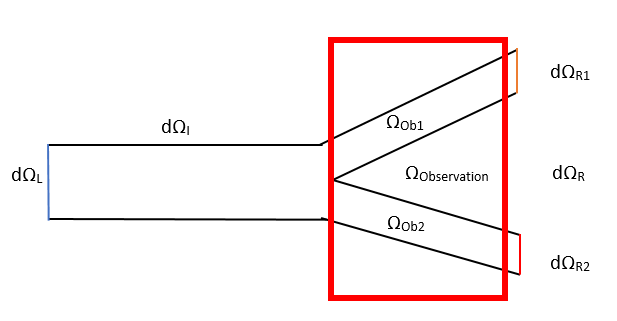
\includegraphics[scale=0.8]{observation.png}
	\caption{Domain of Interest}
	\label{Observation1}
\end{figure}
The first problem of interest is of the form:
\begin{align*}
&\min_{\Sta, w} \quad \frac{1}{2}|| \Sta -\widehat \Sta||^2_{L_2( \Sigma_{Ob})} + \frac{\beta}{2}||w||^2_{L_2(\Sigma)}\\
&\text{subject to:}\\
&\partial_t \rho = \nabla^2 \rho - \nabla \cdot (\rho \mathbf{w}) +\nabla \cdot (\rho \nabla V_{ext}) + \nabla \cdot \int_\Omega \rho(r) \rho(r') \nabla V_2(|r-r'|) dr' + w \quad  \text{in} \quad \Sigma\notag\\
& \rho = \rho_0 \quad \text{at} \quad t=0 \notag\\
& - \mathbf{j} \cdot \nor = \mathbbm{1}_{\partial \Omega_L}( C_{L1}  + C_{L2}\Sta) +\mathbbm{1}_{\partial \Omega_R} ( C_{R1}  + C_{R2}\Sta) +\mathbbm{1}_{\partial \Omega_I} 0 \ \quad \quad\qquad\qquad  \qquad \text{on} \quad \partial \Omega, 
\end{align*}
where $C_{L1}, C_{L2}, C_{R1}$, $C_{R2}$ are constants and $\mathbbm{1}$ is the indicator function of the set of interest. Considering Figure \ref{Observation1}, the stated non-constant flux boundary condition provides the option of describing a non-constant inflow on boundary $\partial \Omega_L$ and a non-constant outflow on $\partial \Omega_R$, while keeping a no flux condition on the rest of the boundary, denoted by $\partial \Omega_I$.
Furthermore, $\mathbf{j}$ satisfies:
\begin{align*}
\mathbf{j}=\nabla \rho - (\rho \mathbf{w}) +(\rho \nabla V_{ext}) +  \int_\Omega \rho(r) \rho(r') \nabla V_2(|r-r'|) dr'.
\end{align*}
Moreover, let $\widehat \Sta$ be defined such that:
\begin{align*}
\widehat \Sta = \mathbbm{1}_{ \Omega_{Ob1}} \tilde \Sta  +\mathbbm{1}_{ \Omega_{Ob2}} 0.
\end{align*}
This describes a desired state where the particle mass accumulates in the observation domain $\Omega_{Ob1}$ and no particles are found in $\Omega_{Ob1}$. Since observations are only taken on $\Omega_{Ob}$, there is no prescribed desired state on $\Omega / \Omega_{Ob}$.\\
The Lagrangian is of the form:
\begin{align*}
\mathcal{L}(\Sta,w,\Adjb,\Adjc ) &=\frac{1}{2} \int_0^T \int_{\Omega_{Ob}} (\Sta - \widehat \Sta)^2 dr dt + \frac{\beta}{2}\int_0^T \int_\Omega w^2 drdt \\
&+ \int_0^T \int_\Omega \bigg( \partial_t \rho - \nabla^2 \rho + \nabla \cdot (\rho \mathbf{w}) -\nabla \cdot (\rho \nabla V_{ext}) \\
&+ \nabla \cdot \int_\Omega \rho(r) \rho(r') \nabla V_2(|r-r'|) -w \bigg) \Adjb dr dt\\
&+ \int_0^T \int_{\partial \Omega} \bigg(  \bigg(-\nabla \rho+ (\rho \mathbf{w}) -(\rho \nabla V_{ext}) -  \int_\Omega \rho(r) \rho(r') \nabla V_2(|r-r'|) dr' \bigg)\cdot \nor\\
&  -\mathbbm{1}_{\partial \Omega_L}( C_{L1}  + C_{L2}\Sta) -\mathbbm{1}_{\partial \Omega_R} ( C_{R1}  + C_{R2}\Sta) -\mathbbm{1}_{\partial \Omega_I} 0 \bigg) \Adjc dr dt.
\end{align*}
The derivative of $\mathcal{L}$ with respect to $\rho$ is, as taken from the extended project, is:
\begin{align*}
&\mathcal{L}_\rho (\rho,{w},\Adjb,\Adjc)h=
\int_\Omega h(T) \Adjb(T) dr\\
&+ \int_0^T \int_\Omega \bigg( \mathbbm{1}_{ \Omega_{Ob}} (\rho- \widehat{\rho})  - \partial_t \Adjb  - \nabla \Adjb \cdot \mathbf{w}  - \nabla^2 \Adjb \notag 
+  \nabla \Adjb \cdot \nabla V_{ext}  \notag \\
&+ \int_\Omega (\nabla  \Adjb(r)+\nabla  \Adjb(r')) \rho(r') \nabla V_2(|r-r'|) dr'+ \int_{\partial \Omega} ( \Adjc(r') - \Adjb(r')) \rho(r')   \frac{\partial V_2(|r-r'|)}{\partial n} dr' \bigg) h dr dt \\
&+  \int_0^T\int_{\partial \Omega}  \bigg(
\bigg(\frac{\partial \Adjb }{\partial n} + \Adjb  \mathbf{w} \cdot \mathbf{n} - \Adjc \mathbf{w} \cdot \mathbf{n}  +  \Adjc \dfrac{\partial V_{ext}}{\partial n} - \Adjb \frac{\partial V_{ext}}{\partial n} + ( \Adjc - \Adjb)  \int_\Omega \rho(r') \frac{\partial V_2(|r-r'|)}{\partial n} dr'\\
& -\mathbbm{1}_{\partial \Omega_L} C_{L2} \Adjc   -\mathbbm{1}_{\partial \Omega_R} C_{R2} \Adjc \bigg)h + \bigg( \Adjc- \Adjb \bigg) \frac{\partial h}{\partial n} \bigg) dr dt =0.
\end{align*}
Then, from appropriate analysis we find that:
\begin{align*}
\Adjc = \Adjb,
\end{align*}
and therefore we get:
\begin{align*}
\mathbbm{1}_{\Omega_{Ob}}(\rho- \widehat{\rho})   - \partial_t  \Adjb  - \nabla \Adjb \cdot \mathbf{w}  - \nabla^2 \Adjb \notag 
+  \nabla \Adjb \cdot \nabla V_{ext}  \notag \\
+ \int_\Omega (\nabla  \Adjb(r)+\nabla  \Adjb(r')) \rho(r') \nabla V_2(|r-r'|) dr' &=0, \quad \text{in} \quad \Sigma, \\
\frac{\partial \Adjb }{\partial n}  -\mathbbm{1}_{\partial \Omega_L} C_{L2} \Adjb   -\mathbbm{1}_{\partial \Omega_R} C_{R2} \Adjb&=0, \quad \text{on} \quad \partial \Omega.
\end{align*}
In particular, this is:
\begin{align*}
\mathbbm{1}_{\Omega_{Ob1}}(\rho- \widehat{\rho}) +\mathbbm{1}_{\Omega_{Ob2}}\rho  - \partial_t  \Adjb  - \nabla \Adjb \cdot \mathbf{w}  - \nabla^2 \Adjb \notag 
+  \nabla \Adjb \cdot \nabla V_{ext}  \notag \\
+ \int_\Omega (\nabla  \Adjb(r)+\nabla  \Adjb(r')) \rho(r') \nabla V_2(|r-r'|) dr' &=0, \quad \text{in} \quad \Sigma, \\
\frac{\partial \Adjb }{\partial n}  -\mathbbm{1}_{\partial \Omega_L} C_{L2} \Adjb   -\mathbbm{1}_{\partial \Omega_R} C_{R2} \Adjb&=0, \quad \text{on} \quad \partial \Omega.
\end{align*}
The gradient equation is:
\begin{align*}
w = \frac{1}{\beta}\Adjb.
\end{align*}
Comparing this to the previous section, it can be observed that the gradient equations have opposite signs. This is due to a different construction of the Lagrangian.




\section{Numerical Methods}
\subsection{Pseudospectral Methods}
- pseudospectral methods (why they are better than others in what we do, what else would be useful, what type of method exactly, how does it work)
\subsection{Multiple Shooting Method}
- multiple shooting background (how is it done in literature, how do we do it)
\subsection{Fixed Point Algorithm}
- Kalise and Burger papers, sweeping algorithms (and our adaptation - or adaptation in next section)\\
- below copy and paste from paper draft. misses intro because ben wrote it -- need to write my own! ++

In the following, we denote the discretized versions of the variables $\rho$, $\adj$ and $\vec{w}$ with $P$, $Q$ and $W$, respectively. Each of these matrices is of the form $A = [\boldsymbol{a_0}, \boldsymbol{a_1}, ... ,\boldsymbol{a_n}]$, where the vectors $\boldsymbol{a_k}$ represent the solutions at the discretized times $k \in 0,1,....,n$, where $n$ is the number of time points. In particular, the first column of $P$, denoted by $\boldsymbol{\rho_0}$, corresponds to the initial condition $\rho(\vec{x},0)$. If the spatial domain is one-dimensional, $P$, $Q$ and $W$ are of size $N \times n$, where $N$ is the number of spatial points. In the two-dimensional case, $P$ and $Q$ are of size $(N_1N_2) \times n$, where $N_1$ is the number of spatial points in the direction of $x_1$ and $N_2$ the points along the $x_2$ axis. Generally, $N_1 = N_2$. The discretized control $W$ for linear control problems is also $(N_1N_2) \times n$ dimensional, while it is $(2N_1N_2) \times n$ dimensional for nonlinear control problems. This is due to the fact that the control is represented by a vector field, when applied nonlinearly.
\\
\\
The optimization algorithm is initialized with a guess for the control, $W^{(0)}$. Then, in each iteration, denoted by $i$, the following steps are computed:
\vspace{0.1cm}
\begin{enumerate}
	\item Starting with a guess for the control $W^{(i)}$ as input variable, the corresponding state $P^{(i)}$ is found by solving the forward equation.
	\item In a next step, the value of the adjoint, $Q^{(i)}$, is established by computing the adjoint equation, using $W^{(i)}$ and $P^{(i)}$ as inputs. Since $P^{(i)}$ contains the solution for all discretized times $k \in 0,1,...,n$, this circumvents issues resulting from the non-local coupling in time, mentioned in Section \ref{sec:Method_PseudospectralPDECO}. As illustrated in the same section, time is reversed in the adjoint equation, so that the result is a matrix $\tilde{Q}^{(i)} =  [\boldsymbol{\adj_n},\boldsymbol{\adj_{n-1}}, ..., \boldsymbol{\adj_1} ]$. The columns of $\tilde{Q}^{(i)}$ are permuted to obtain the solution  $Q^{(i)}$.
	\item The gradient equation is solved, given the solutions $P^{(i)}$ and $Q^{(i)}$. This results in a new value for the control, $W^{(i)}_g$.
	\item  The convergence of the optimization scheme is measured by computing the error between $W^{(i)}$ and $W^{(i)}_{g}$. The error measure, $\mathcal{E}$, is discussed in detail in Section \ref{sec:Method_Validation}. 
	\begin{itemize}
		\item  If this error is lower than a set tolerance, the optimality system is self-consistent. This implies that the solution triplet ($\bar{P},\bar{W},\bar{Q}$) solves the (discretized) optimality system, and is therefore an optimal solution to the PDE-constrained optimization problem of interest.
		\item If the error is above the optimality tolerance, step 5 is executed.
	\end{itemize}
	\item Finally, the update $W^{(i+1)}$ is a linear combination of the current guess $W^{(i)}$, and the value obtained in step 3, $W^{(i)}_{g}$, employing a mixing rate $\lambda \in [0,1]$:
	\begin{align*}
	W^{(i+1)} = (1-\lambda)W^{(i)} + \lambda W^{(i)}_{g}.
	\end{align*}
	The guess for the control is updated from $W^{(i)} $ to $W^{(i+1)} $ and steps 1-5 are repeated until the method converges. 
\end{enumerate}
\vspace{0.3cm}
The update scheme in step 5, with mixing rate $\lambda$, is known to stabilise fixed point methods, ++Ben to add references++. Typical values of $\lambda$, which provide stable convergence, lie between $0.1$ and $0.001$. Throughout this paper, $\lambda =0.01$, unless stated otherwise. This mixing scheme is equivalent to the updating scheme presented in~\cite{Burger1}. 
Note that, while the solutions $P^{(i)}$ and $Q^{(i)}$ change in each iteration, the initial condition $\boldsymbol{\rho_0}$ and final time condition $\boldsymbol{\adj_n}$ remain unchanged throughout the process. Therefore, the only variable inducing a change in the solution is $W^{(i)}$.

++ Add something about errors -- mention to see below? ++

- showing why running ODE solver piecewise is more accurate than on the whole time line\\
- Chebyshev time points vs equispaced time grid for spectral accuracy\\
\\

- fixed point method: explain where it came from, adding mixing rate and why and that burger and ours are the same (derivation?)\\
- explain general functionality of the algorithm, the different input options, how the optimization algorithm works, what can be changed (e.g. norms, solvers, etc), what up to date is the fastest method, what is the most robust, etc. (here maybe the PDECO input PDF is helpful?)


\subsection{Inbuilt Matlab functions}
\subsubsection{The ODE solver}
- discuss different ODE solvers and which one is best for this and why
\subsubsection{The inbuilt optimization solver}
- here maybe some of the 'fsolveResearch' stuff?\\
- discuss how fsolve works (the review done on it etc) and what alternative is there in the literature\\

\section{Investigating Functionality of the Optimization Algorithms}
- Multiple shooting\\
- Fixed Point\\
- find a way to separate but join the following subsections for the two solvers\\
\subsection{Error measures}
- L2Linfinity Relative\\
- Pointwise Relative\\
- Absolute L1\\
- other?\\
- argue why relative is better, why one error measure is better than others etc
\subsubsection{L2Linfinity Relative Error}
++ Copied from paper, needs context ++
All errors in Section \ref{sec:Method_Validation} and Section \ref{sec:Expts} are calculated between a variable of interest, $y$, and $y_R$, the reference value that $y$ is compared to. When measuring convergence of the fixed point scheme, described in Section \ref{sec:Method_Solver}, $y = W^{(i)}_g$ and $y_R = W^{(i)}_i$. Alternatively, when investigating a known test problem, as done in Appendix \ref{app:TestProblems}, $y$ is a numerical solution and $y_R$ is an exact solution. The error measure $\mathcal{E}$ is composed of an $L^2$ error in space and an $L^\infty$ error in time. The relative $L^2$ error in the spatial direction is:
\begin{align*}
\mathcal{E}_{Rel}(t) = \frac{|| y(x,t) - y_{R}(x,t)||_{L^2(\Omega)} }{||y_R(x,t) + 10^{-10}||_{L^2(\Omega)}},
\end{align*}
where the small additional term on the denominator prevents division by zero.
Furthermore, the absolute $L^2$ error is:
\begin{align*}
\mathcal{E}_{Abs}(t) = || y(x,t) - y_R(x,t)||_{L^2(\Omega)}.
\end{align*}
Then, an $L^\infty$ error in time is taken of the minimum of $\mathcal{E}_{Rel}$ and $\mathcal{E}_{Abs}$, to obtain the error of interest:
\begin{align*}
\mathcal{E} = \max_{t \in [0,T]}\left[\min\left(\mathcal{E}_{Rel}(t), \mathcal{E}_{Abs}(t)\right)\right].
\end{align*}
The minimum between absolute and relative spatial error is taken to avoid choosing an erogenously large relative error, caused by division of one small term by another.

As a benchmark, we compared the fixed point scheme to Matlab's inbuilt \texttt{fsolve} function. It uses the trust-region-dogleg algorithm, see~\cite{Powell1}, to solve the optimality system of interest. While it is very robust, it is also much slower than the fixed point method, which works reliably for the types of problems considered in this paper. A comparison is given in Appendix \ref{app:fsolveComparison}. Numerical results for specific test problems with exact solutions are supplied in Appendix \ref{app:TestProblems}. Further tests to validate the method are presented in Appendix \ref{app:TestProblemsPerturbed}.


\subsection{Exact Solutions}
- all four problems \\
- mention that $w \sim \frac{1}{\beta}$ doesn't work well - should be on $p$ or both $\rho$ and $p$ instead \\
- compare different choices of exact solutions, i.e. linear, polynomial, exponential time; polynomial and trigonometric space \\
- show the performance of the polynomial vs. exponential for interpolation (this may have to go to 'tests on other parts of the code') \\
\subsection{Validation against different solvers}
- compare results of the same problem for fsolve, picard and fixed point method\\
- compare the different solvers. Compare how they measure convergence and which may do better or how they differ in general.\\
\\
\\

Example 1 in Section \ref{sec:Examples1d} is considered to compare the computational time taken of the fixed point algorithm and the inbuilt Matlab function \texttt{fsolve}. Note that the comparison is slightly impacted by the fact that convergence is measured differently in these two numerical methods. However, a general comparison can be made regarding the efficiency of the two approaches.
We choose $n=20$, $N=30$, the ODE solver tolerance is set to be $10^{-8}$, the optimality tolerance is $10^{-4}$ and $\beta = 10^{-3}$. 
As can be seen in Table \ref{TabA3:Prob11}, the running time of the fixed point algorithm is considerably faster than for \texttt{fsolve}, while the resulting values of the cost functional remain the same. This can be confirmed by comparing the number of function evaluations for each method, which is an important measure when dealing with large systems, such as the two-dimensional problems discussed in this paper, since each iteration is costly for large problems. The differences in $\rho$ and $\adj$ are broadly in line with the optimality tolerance, however the control differs more, because $\mathbf{w}$ is updated using the optimal values of $\rho$ and $\adj$. 
%
\begin{table}
\begin{tabular}{ | c | c || c | c | c ||}
\hline
\multicolumn{2}{|c||}{} & Fixed Point & \texttt{fsolve} & Difference   \\
\hline
\hline
 & $\mathcal{J}_{uc}$ & $\numprint{0.0438}$ & $\numprint{0.0438}$ &   \\
 & $\mathcal{J}_{c}$ & $\numprint{0.0011}$ & $\numprint{0.0011}$ &   \\
 & \texttt{Iter} (\texttt{funcEval}) & $\numprint{670}$ ($\numprint{670}$)  & $\numprint{38}$ ($\numprint{31959}$)  &   \\
$\kappa =-1$ & Time taken (s) & $\numprint{2.4939e+2}$ & $\numprint{9.1546e+3}$ &   \\
 & $\mathcal{E}_{\rho_{Diff}}$ & & &$\numprint{1.1348e-3}$  \\
 & $\mathcal{E}_{\adj_{Diff}}$ & & &$\numprint{7.2742e-5}$  \\
 & $\mathcal{E}_{\mathbf{w}_{Diff}}$ & & & $\numprint{7.6725e-2}$  \\
\hline
 & $\mathcal{J}_{uc}$ & $\numprint{0.0434}$ & $\numprint{0.0434}$ &   \\
 & $\mathcal{J}_{c}$ & $\numprint{0.0020}$ & $\numprint{0.0020}$ &   \\
 & \texttt{Iter} (\texttt{funcEval}) & $\numprint{654}$ ($\numprint{654}$)  & $\numprint{38}$ ($\numprint{34239}$)  &   \\
$\kappa =1$ & Time taken (s) & $\numprint{3.3794e+2}$ & $\numprint{1.0167e+4}$ &   \\
 & $\mathcal{E}_{\rho_{Diff}}$ & & &$\numprint{3.0610e-4}$  \\
 & $\mathcal{E}_{\adj_{Diff}}$ & & &$\numprint{4.8701e-5}$  \\
 & $\mathcal{E}_{\mathbf{w}_{Diff}}$ & & & $\numprint{8.9056e-3}$  \\
\hline
\end{tabular}
\caption{Comparison of the outputs of the fixed point method, with those obtained using \texttt{fsolve}.}
\label{TabA3:Prob1}
\end{table} \label{TabA3:Prob11}


\subsection{Perturbing $\hat \rho$}
- taking $\rho$ IC/IG of exact solution with $\beta_1$ and all other choices exact for $\beta_2$ and see what happens. \\
- other tests that change $\hat \rho$ instead of $w$. Can't remember exactly
\subsection{Perturbing $w$}
- discuss why the perturbation has to be smooth (in general and wrt the initial condition, give examples, error plots) AND check if that's still true given the knowledge on advection dominance and size of the problem\\
- perturbing in time \\
- perturbing in space \\
- perturbing in time and space \\
- symmetric/ asymmetric, different strengths\\
- relationship between this and the advection dominance\\
- show interpolation error in perturbed $w$\\
- perturb $\rho$ and show interpolation error there too\\
\\
\\

As detailed in Section \ref{sec:Method_SolverFP}, it is necessary to provide an initial guess for the control $\mathbf{w}$ to start the optimization routine. Therefore, one way of validating the numerical method is to perturb the exact solution for $\mathbf{w}$, taken from a test problem with analytic solution, and use this as an initial guess in the optimization solver. In the first iteration, the solutions for $\rho$ and $\adj$ differ from the exact solution. The optimization method then converges to the exact, optimal solution. We consider an exact solution for the overdamped flow control problem \eqref{eqn:ADFlowOCP}, with no-flux boundary conditions, and no particle interaction term. This specific exact solution can be found in our paper's supplementary material (Section A), called Test Problem 2. 
The following two perturbation functions are considered. The first perturbation is in time only and is defined as:
\begin{align*}
g(t) &= \frac{1}{2} f(t-t_0, a) \times f(t-t_0, -a)\\
&= \frac{1}{2} \frac{e^{-a/(t-t_0)}}{e^{-a/(t-t_0)} + e^{-a/(1-t -t_0)}} \times \frac{e^{a/(t-t_0)}}{e^{a/(t-t_0)} + e^{a/(1-t - t_0)}},
\end{align*}
and normalised by:
\begin{align*}
\tilde g(t) = \frac{g(t)}{\max{|{g(t)}|}}.
\end{align*}
A similar perturbation can be done in space, taking into account the difference in length of spatial and time domains:
\begin{align*}
h(x) &= \frac{1}{2} f(x-x_0, 2a) \times f(x-x_0, -2a)\\
&= \frac{1}{2} \frac{e^{-2a/(x-x_0)}}{e^{-2a/(x-x_0)} + e^{-2a/(1-x-x_0)}} \times \frac{e^{2a/(x-x_0)}}{e^{2a/(x-x_0)} + e^{2a/(1-x-x_0)}}.
\end{align*}
Again, this is normalised:
\begin{align*}
\tilde h(x) = \frac{h(x)}{\max{|{h(x)}|}}.
\end{align*}
These perturbation functions are chosen such that the perturbation is smooth and respects the initial condition for $\rho$, as well as the final time condition for $\adj$, by not changing the first or final time point. If this is not respected, the algorithm converges up to a point and then diverges, since the boundary conditions in time cannot be matched.
The considered perturbations are applied to the exact solution of the control, $\mathbf{w}_{ex}$, as follows:
\begin{align*}
\mathbf{w}_{pert1} &= \mathbf{w}_{ex}(1+ \epsilon \tilde g(t))\\
\mathbf{w}_{pert2} &= \mathbf{w}_{ex}(1+ \epsilon \tilde g(t) \tilde h(x)),
\end{align*}
where $a = 0.7$, $x_0 = t_0 = -0.01$ and the perturbation strength is either $\epsilon = 0.1$ or $\epsilon = 0.5$.
The chosen number of points is $N =30$ and $n=20$, the ODE tolerances are $10^{-8}$ and the optimality tolerance is $10^{-4}$. The mixing rate for the optimization solver is $\lambda = 0.01$.
The results presented in Table \ref{TabA2:Prob11} show the initial error in $\mathbf{w}$, $\mathcal{E}_{\mathbf{w}_{uc}}$, and the final errors in $\mathbf{w}$, $\rho$ and $\adj$, measured in the norm presented in Section \ref{sec:ErrorMeasure}, with respect to the exact solution. The initial error $\mathcal{E}_{\mathbf{w}_{uc}}$ is proportional to the perturbation strength $\epsilon$. The final errors for $\mathbf{w}$ and $\rho$ and $\adj$ are mostly within the specified optimality tolerance regardless of the perturbation strength and location. 

\begin{table}
\begin{tabular}{ | c | c || c | c | c | c ||}
\hline
  \multicolumn{2}{|c||}{} & $\beta = 10^{-3}$ & $\beta = 10^{-1}$ & $\beta = 10^{1}$ & $\beta = 10^{3}$  \\
\hline
\hline
\multirow{4}{*}{$0.1 \tilde g(t)$} & $\mathcal{E}_{\mathbf{w}_{uc}}$ & $\numprint{1.0000e-1}$ & $\numprint{1.0000e-1}$ & $\numprint{1.0000e-1}$ & $\numprint{1.0000e-1}$ \\
 & $\mathcal{E}_{\mathbf{w}_c}$ & $\numprint{5.3770e-5}$ & $\numprint{5.2340e-5}$ & $\numprint{5.2201e-5}$ & $\numprint{5.2203e-5}$ \\
 & $\mathcal{E}_{\rho}$ & $\numprint{1.1396e-5}$ & $\numprint{7.8597e-5}$ & $\numprint{7.8595e-5}$ & $\numprint{7.8597e-5}$ \\
 & $\mathcal{E}_{\adj}$ & $\numprint{2.7854e-5}$ & $\numprint{2.7836e-4}$ & $\numprint{5.7043e-4}$ & $\numprint{5.7045e-4}$ \\
\hline
\multirow{4}{*}{$0.5 \tilde g(t)$} & $\mathcal{E}_{\mathbf{w}_{uc}}$ & $\numprint{5.0000e-1}$ & $\numprint{5.0000e-1}$ & $\numprint{5.0000e-1}$ & $\numprint{5.0000e-1}$ \\
 & $\mathcal{E}_{\mathbf{w}_c}$ & $\numprint{2.1970e-4}$ & $\numprint{2.1747e-4}$ & $\numprint{2.1735e-4}$ & $\numprint{2.1735e-4}$ \\
 & $\mathcal{E}_{\rho}$ & $\numprint{2.4256e-5}$ & $\numprint{2.2878e-4}$ & $\numprint{2.2878e-4}$ & $\numprint{2.2879e-4}$ \\
 & $\mathcal{E}_{\adj}$ & $\numprint{3.3247e-5}$ & $\numprint{3.3227e-4}$ & $\numprint{6.8088e-4}$ & $\numprint{6.8090e-4}$ \\
\hline
\multirow{4}{*}{$0.1 \tilde h(x)$} & $\mathcal{E}_{\mathbf{w}_{uc}}$ & $\numprint{8.5568e-2}$ & $\numprint{8.5568e-2}$ & $\numprint{8.5568e-2}$ & $\numprint{8.5568e-2}$ \\
 & $\mathcal{E}_{\mathbf{w}_c}$ & $\numprint{5.3700e-5}$ & $\numprint{5.2250e-5}$ & $\numprint{5.2100e-5}$ & $\numprint{5.2103e-5}$ \\
 & $\mathcal{E}_{\rho}$ & $\numprint{1.1704e-5}$ & $\numprint{7.7973e-5}$ & $\numprint{7.7969e-5}$ & $\numprint{7.7968e-5}$ \\
 & $\mathcal{E}_{\adj}$ & $\numprint{2.6426e-5}$ & $\numprint{2.6387e-4}$ & $\numprint{5.6982e-4}$ & $\numprint{5.6984e-4}$ \\
\hline
\multirow{4}{*}{$0.5 \tilde h(x)$} & $\mathcal{E}_{\mathbf{w}_{uc}}$ & $\numprint{4.2784e-1}$ & $\numprint{4.2784e-1}$ & $\numprint{4.2784e-1}$ & $\numprint{4.2784e-1}$ \\
 & $\mathcal{E}_{\mathbf{w}_c}$ & $\numprint{2.1203e-4}$ & $\numprint{2.0982e-4}$ & $\numprint{2.0967e-4}$ & $\numprint{2.0968e-4}$ \\
 & $\mathcal{E}_{\rho}$ & $\numprint{2.2565e-5}$ & $\numprint{2.1275e-4}$ & $\numprint{2.1274e-4}$ & $\numprint{2.1275e-4}$ \\
 & $\mathcal{E}_{\adj}$ & $\numprint{3.0225e-5}$ & $\numprint{3.0219e-4}$ & $\numprint{6.1920e-4}$ & $\numprint{6.1923e-4}$ \\
\hline
\end{tabular}
\caption{Error measures for $\mathbf{w}_{uc}$, $\mathbf{w}_{c}$, $\rho$, and $\adj$, for four perturbation strategies for $\mathbf{w}$, and a range of $\beta$.}
\label{TabA2:Prob1}
\end{table} \label{TabA2:Prob11}

\subsection{Investigating changing $n$ and $N$}
- for both FW and optimization problem investigate how the error changes with the number of points\\
- investigate effect of beta and of tolerance settings\\

\subsection{Investigating changing tolerances}
- for both FW and optimization problem investigate how error changes with ODE tolerances (and include how it changes with not using the same tolerances for both RelTol and AbsTol)\\
- investigate interplay between this and number of points and beta
- for optimization problem do this for both ODE tolerances and optimality tolerances (whatever they are - do for different solvers)\\
- discuss how to choose tolerances given things such as interpolation errors and such.


\subsection{Investigating $\lambda$}
- what range of values is suitable\\
- interplay with $\beta$\\
- adaptive for different problems\\
- include here a study on how the convergence works: i.e. is it 'linear' over iterations, or is it behaving in any certain way. use this to justify adaptive approach
\subsection{Choice of $\hat \rho$}
- stationary vs moving\\
- achievable or not\\
- satisfying BCs and IC
\subsection{Choice of Initial Guess for $\adj$ (Multiple Shooting)}
- explain what has to be satisfied\\
- one idea: integrate from the gradient eqn. for initial guess of w. Check that this is still tricky with our new understanding of the exact solutions (too large, advection dominance, etc). \\
- other idea: one Kalise step to come up with p.\\
- show how much or how little the choice of initial guess for $p$ matters in toy examples.\\
- for both IGs show whether different IGs converge to the global minimum/ exact solution or whether it converges to some local minimum
\subsection{The relationship between diffusion and advection}
- investigate the size of the two terms \\
- when do different problems break because of advection dominance\\
- how does the interaction term come into this\\
- break something that works and fix something that doesn't, show breaking point and whether the relationship is abrupt or linear or what else\\
-check time interpolation for fixed x, does it get worse with larger solutions?
- Show example where it breaks eg 2D example with too steep desired state (advection dominance/ too steep gradients)\\
- investigate going from coarse grid to fine grid to push accuracy of solutions. see if it's to do with advection or ODE solver limitations.

\subsection{Tests on other parts of the code}
- showing why running ODE solver piecewise is more accurate than on the whole time line\\
- Chebyshev time points vs equispaced time grid for spectral accuracy (demo somewhere)
\subsubsection{Investigating interpolation errors}
- investigate the effect of interpolation error in interplay with tolerances, and number of points, and other factors.\\
- can be in link with perturbing $w$ too maybe?

\section{Examples}
- Neumann Flow\\
- Mass conservation, $\rho$ size $1$ for probability distribution\\
- symmetric\ asymmetric\\
- with interaction term \\
- 1D/2D \\
\\
- Dirichlet Flow \\
- Dirichlet Flow with $\rho$ size $1$ -- non-zero BCs ($0.5$ instead/ $0.25$ in 2D)
- Force Control (Dirichlet/Neumann) \\
- show how $w$ from zero in FW problem acts to achieve $\hat \rho$ working against or with interaction\\
- does the control focus on where the mass of the particles is?\\
- choose the examples in a way that each of them is making a point\\
- two peaks example and example with gaussian asymmetric $\hat \rho$\\
- plot space and time as surface plot (with colours) to show how the solution changes with time in 1D\\

++ See paper draft, section 5 (version from before Ben and John change things) for some inspiration on this. ++ \\
\\
\\
+++  copied from paper draft. fix +++
In order to solve the optimal control problems \eqref{AdvDiff} and \eqref{AdvDiff_Linear}, some inputs must be provided. The desired state $\widehat \rho$, the PDE source term $f$, and the external potential $V_{ext}$ must be given. Furthermore, an initial condition for $\rho$, the final time condition for $\adj$ and an initial guess for the control $\vec{w}$ have to be be specified. 
The interaction kernel (++ terminology? ++) is of the form:
\begin{align*}
\vec{K} = \nabla V_2, \qquad V_2 = e^{-x^2}.
\end{align*}
Three interaction strengths are considered in this section. Firstly, each problem is solved without an interaction term present ($\gamma = 0$). Then, the considered problem is solved with an order one attractive interaction term ($\gamma = -1$) and an order one repulsive interaction term ($\gamma = 1$), respectively. Initially, the control $\vec{w}$ is set to zero. It is then investigated how the control changes from this baseline, influenced by the different interaction strengths. 
Initially the forward PDE is solved, using the initial configuration $\vec{w}=0$ and the cost functional $J$ is evaluated at this initial state and denoted by $J_I$. Note that no optimization methods are used to derive this value. We then expect that applying the optimization method lowers the value of the cost functional, which we aim to minimize. 
In particular, the value of the optimal cost functional, denoted by $J_O$, is lower the more control is allowed to enter the system though the optimization process. 
This depends on the value of the regularization parameter $\beta$ and it is expected that the control will increase with decreasing $\beta$, since the cost functionals in problems \eqref{AdvDiff} and \eqref{AdvDiff_Linear} allow for a larger control with smaller $\beta$. 

In the following examples, the domain considered is $\Omega \times [0,T] = [-1,1] \times [0,1]$. The number of spatial points is $N=30$ in one-dimensional examples, $N_1 = N_2 = 30$ in two-dimensional examples, and the number of time points is $n=20$, unless stated otherwise. The tolerances in the ODE solver are set to $10^{-8}$ and the tolerance for the convergence of the optimization algorithm is $10^{-4}$. The mixing parameter $\lambda$ is $0.01$, unless stated otherwise.
\subsection{Nonlinear control problems with an additional nonlocal integral term in 1D} \label{sec:Examples1d}
Examples of solving Problem \eqref{AdvDiff}, with 'no-flux type'/Neumann boundary conditions \eqref{NoFlux} and Dirichlet boundary conditions \eqref{Dirichlet} are given in this section. 
 
\subsubsection{Neumann boundary conditions, Example 1}	 
The chosen inputs for this example are:
\begin{align*}
&\widehat \rho = \frac{1}{2}(1-t) + t\bigg(\frac{1}{2}\sin(\pi (y - 2)/2) + \frac{1}{2}\bigg),\\
&\rho_{0} = \frac{1}{2}, \ \
\adj_{T} = 0, \ \
\vec{w} = \vec{0}, \ \ 
f =0,\ \
V_{ext} =0.
\end{align*}	
The value of the cost functional for the initial configuration ($J_{I}$), where $\vec{w} =0$, is compared with the optimized case ($J_{O}$) for different values of $\beta$ and for each of the interaction strengths in Table \ref{TabS5:Prob1}. It can be observed that in all cases $J_{O}$ is lower or equal value to $J_{I}$. The lowest values of $J_{O}$ will be observed for the smallest $\beta$ value considered. At large values of $\beta$, applying control is heavily penalised and the optimal control approaches zero, which coincides with the uncontrolled case. Furthermore, this is reflected in the number of iterations, which is small when $\beta$ is large, and vice versa. This is explained by the fact that if applying control is penalized heavily, then $\vec{w} = 0$ is a better initial guess, and less iterations are needed to find the optimal solution, than when $\beta$ is small and more control is allowed.

 The desired state $\widehat \rho$, and the uncontrolled state $\rho$ for $\gamma =1$ and $\gamma = -1$ are shown in Figure \ref{Ex12DN1}. These two variables are independent of $\beta$. However, $\rho$ changes considerably with the choice of interaction strength $\gamma$, accumulating mass in the centre of the domain for attractive interactions and at the boundary for repulsive interactions. The optimal states $\rho$ for $\gamma = 1,0,-1$ and corresponding optimal controls, with $\beta = 10^{-3}$, are shown in Figure \ref{Ex12DN2}. 
It can be observed that in the case of $\beta = 10^{-3}$, the optimal state $\rho$ is very similar to $\hat \rho$, regardless of the choice of interaction. However, the corresponding control plot reveals that the control has to be applied differently in each case to account for the interaction effects. In general, the control is largely applied on the right half of the spatial domain, to carry mass to the left, where the desired state dictates it to be, as can be seen when $\gamma = 0$. However, when the particle interaction is repulsive, the control is moving some of the particle mass away from the boundary at $x=-1$ to correct for the repulsive particles accumulating there without control present, as illustrated in Figure \ref{Ex12DN1}. In the attractive case, the control corrects by carrying some mass to the boundary at $x=1$, since the uncontrolled particle density is clustered in the middle of the domain in this case, compare to Figure \ref{Ex12DN1}.
\begin{figure}[h]
	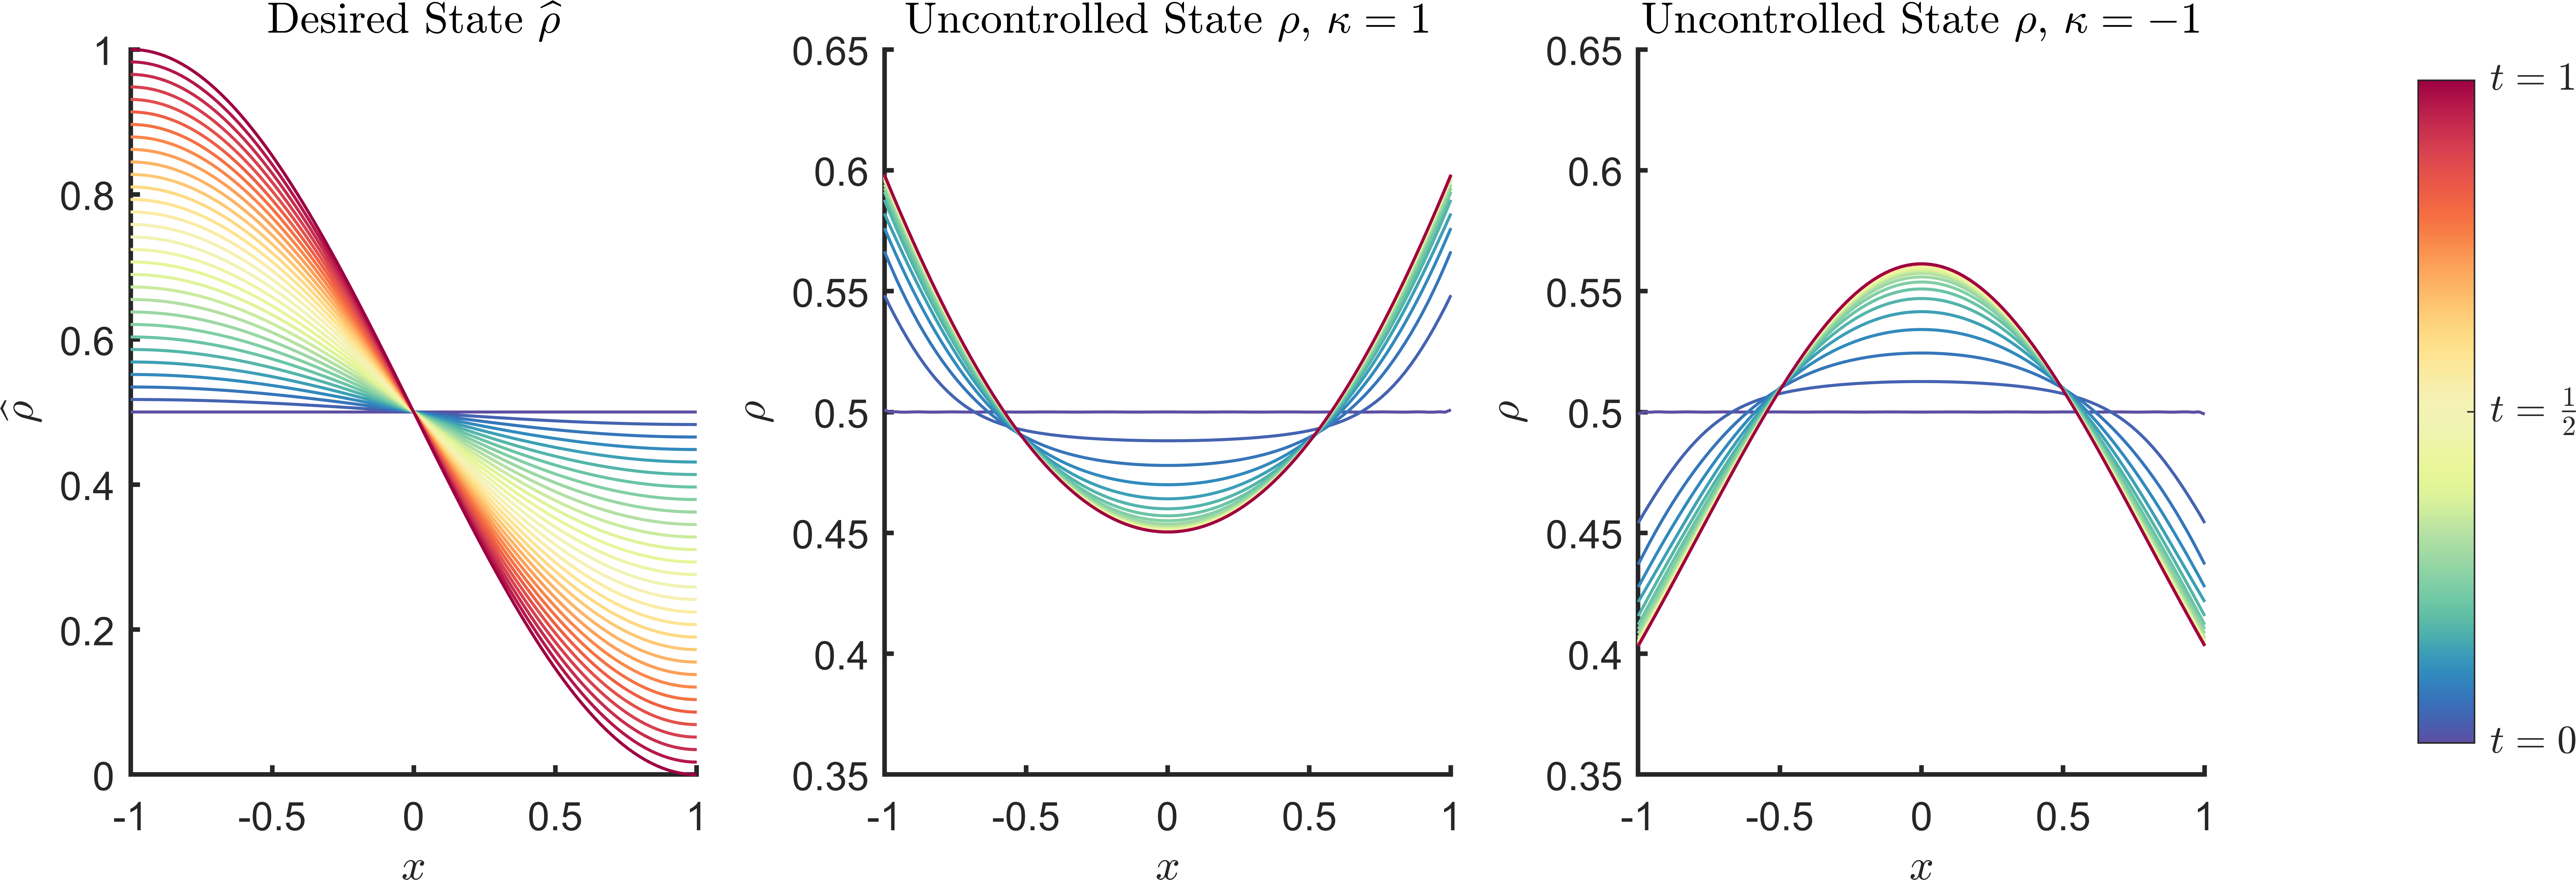
\includegraphics[scale=0.05]{Figure1.png}
	\caption{Example 1, desired state $\widehat \rho$ and uncontrolled state $\rho$ at $\gamma =1$ and $\gamma =-1$}
	\label{Ex12DN1}
\end{figure}
\begin{figure}[h]
	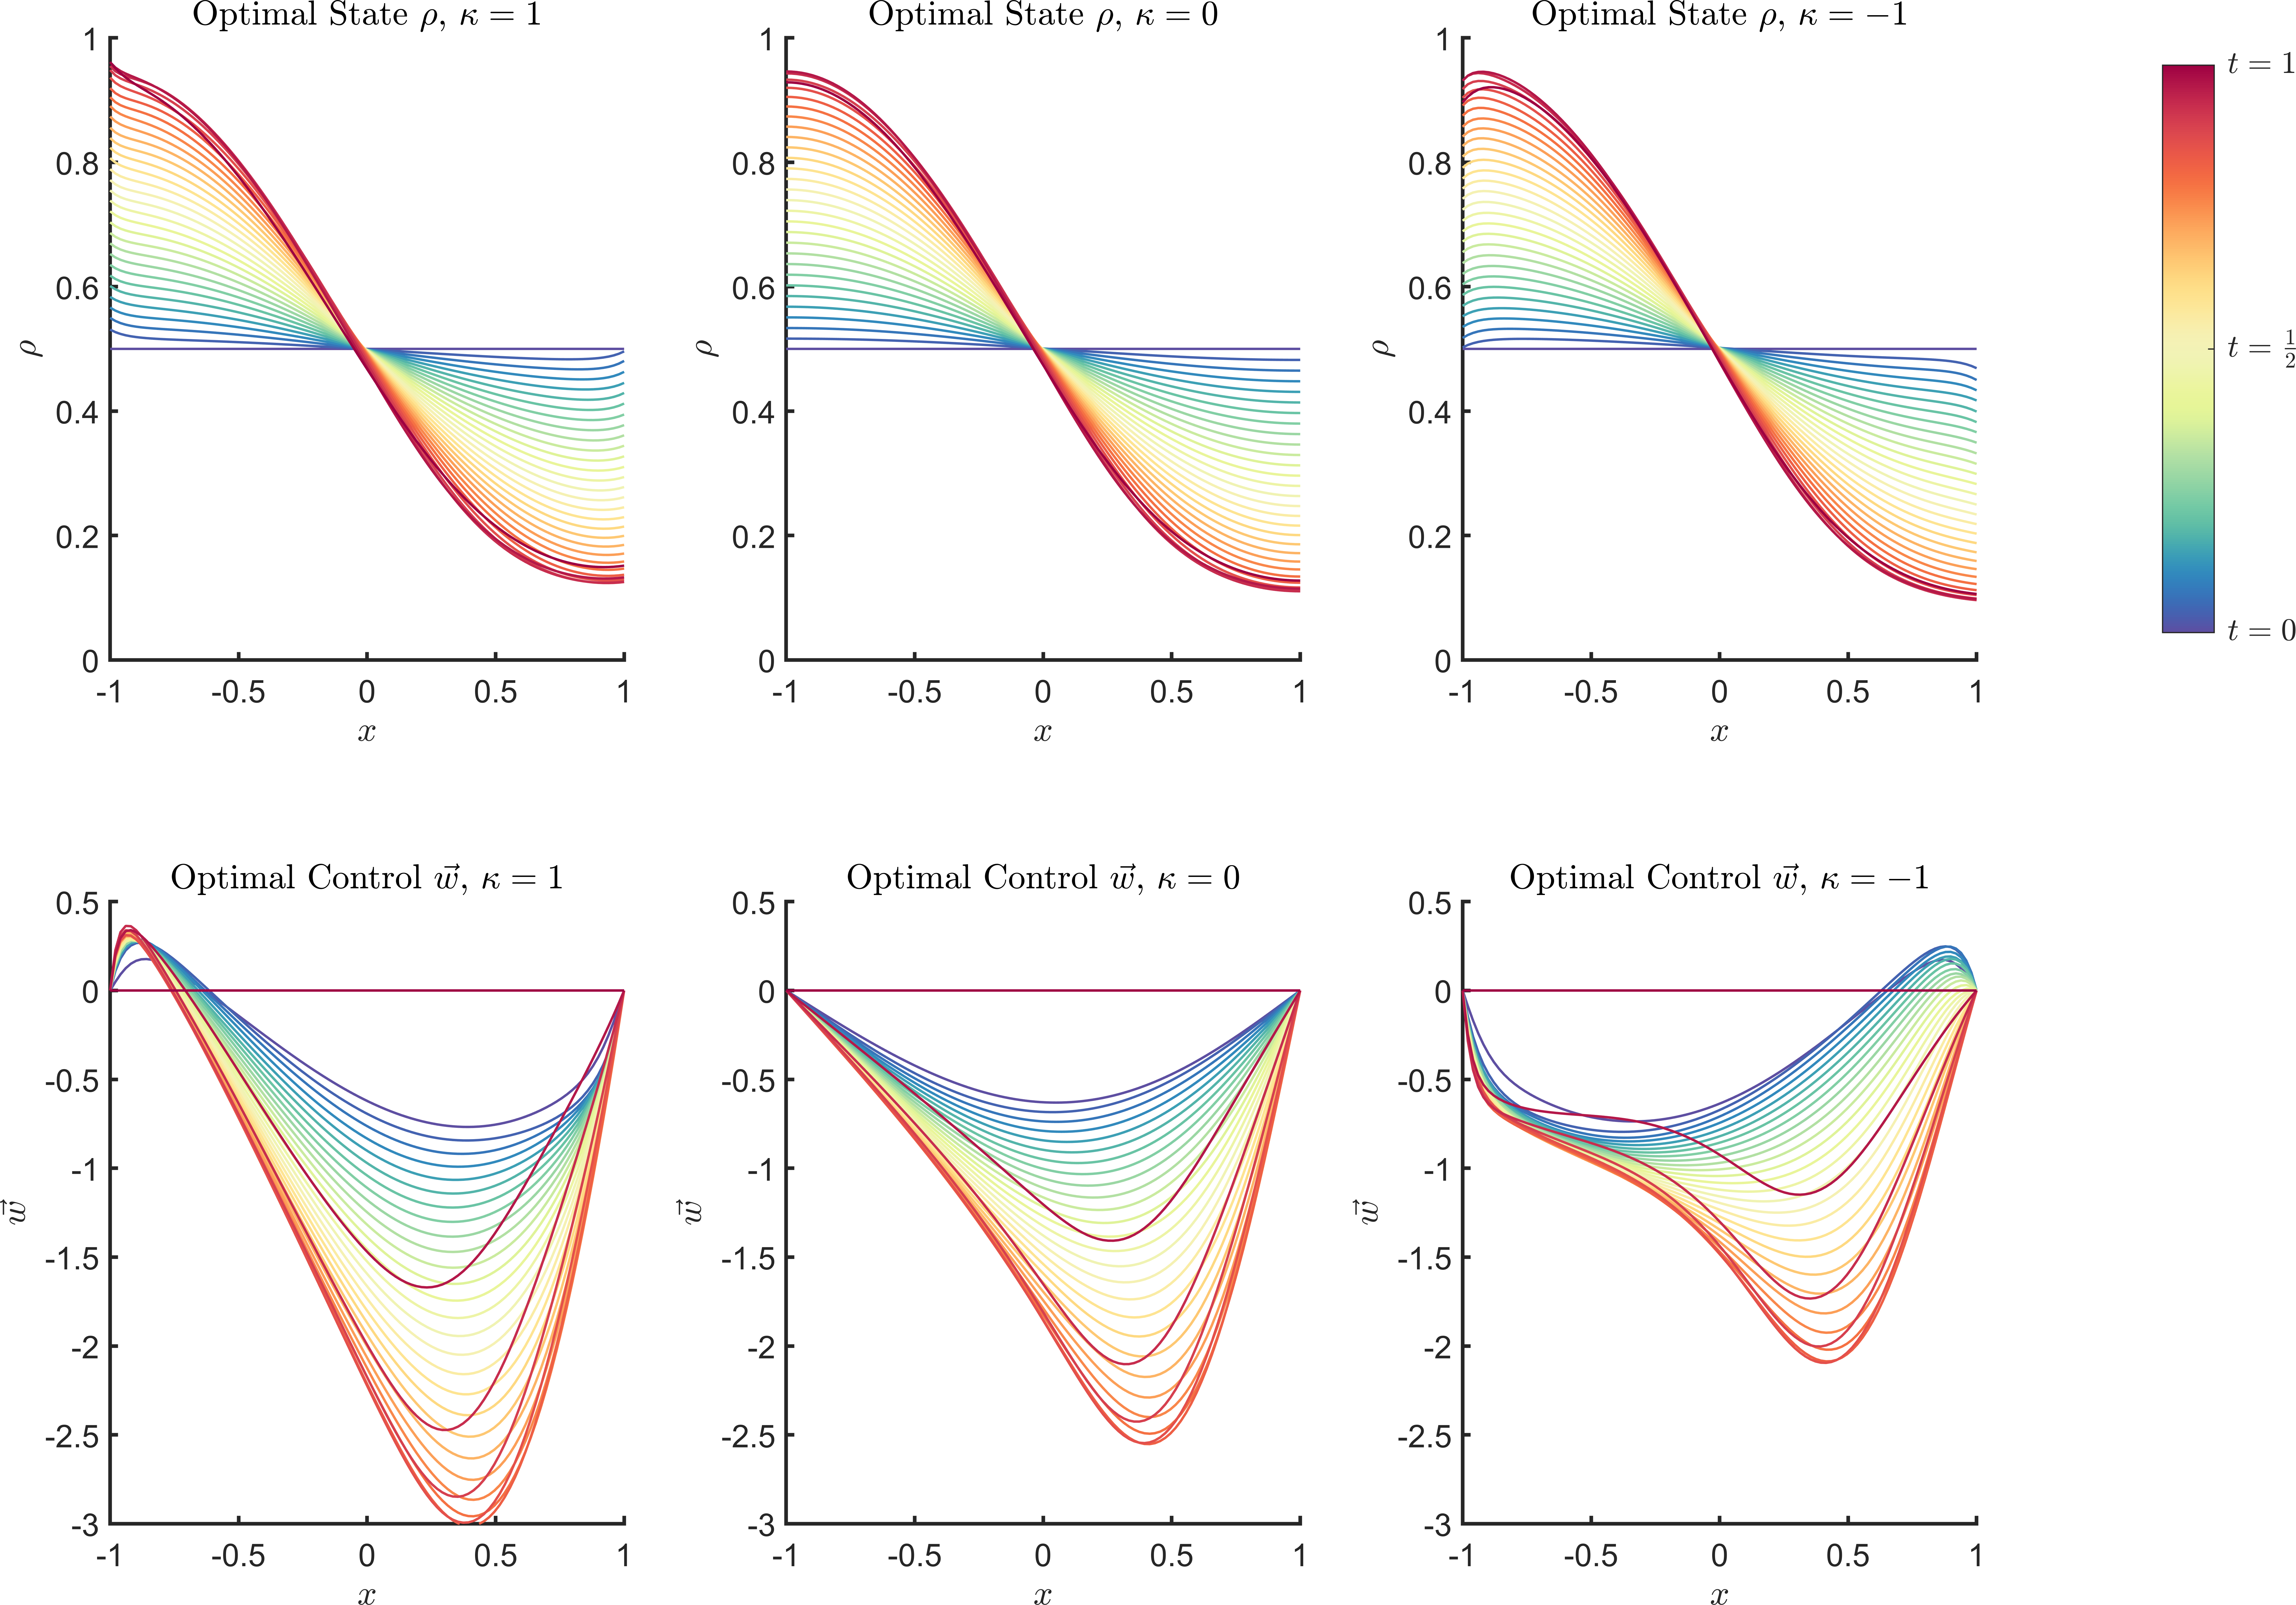
\includegraphics[scale=0.05]{Figure2.png}
	\caption{Example 1, optimal state $\rho$ and the corresponding optimal control $\vec{w}$ for $\gamma = 1,0,-1$, $\beta = 10^{-3}$.}
	\label{Ex12DN2}
\end{figure}

\begin{table}
\begin{tabular}{ | c | c || c | c | c | c ||}
\hline
\multicolumn{2}{|c||}{}& $\beta = 10^{-3}$ & $\beta = 10^{-1}$ & $\beta = 10^{1}$ & $\beta = 10^{3}$  \\
\hline
\hline
 & $\mathcal{J}_{uc}$ & $\numprint{0.0438}$ & $\numprint{0.0438}$ & $\numprint{0.0438}$ & $\numprint{0.0438}$ \\
$\kappa= \numprint{-1}$  & $\mathcal{J}_c$ & $\numprint{0.0011}$ & $\numprint{0.0267}$ & $\numprint{0.0435}$ & $\numprint{0.0438}$ \\
& \texttt{Iter} & $\numprint{670}$ & $\numprint{650}$ & $\numprint{449}$ & $\numprint{1}$ \\
\hline
 & $\mathcal{J}_{uc}$ & $\numprint{0.0417}$ & $\numprint{0.0417}$ & $\numprint{0.0417}$ & $\numprint{0.0417}$ \\
$\kappa= \numprint{0}$  & $\mathcal{J}_c$ & $\numprint{0.0014}$ & $\numprint{0.0283}$ & $\numprint{0.0415}$ & $\numprint{0.0417}$ \\
& \texttt{Iter} & $\numprint{665}$ & $\numprint{656}$ & $\numprint{434}$ & $\numprint{1}$ \\
\hline
 & $\mathcal{J}_{uc}$ & $\numprint{0.0434}$ & $\numprint{0.0434}$ & $\numprint{0.0434}$ & $\numprint{0.0434}$ \\
$\kappa= \numprint{1}$  & $\mathcal{J}_c$ & $\numprint{0.0020}$ & $\numprint{0.0322}$ & $\numprint{0.0432}$ & $\numprint{0.0434}$ \\
& \texttt{Iter} & $\numprint{654}$ & $\numprint{682}$ & $\numprint{422}$ & $\numprint{1}$ \\
\hline
\end{tabular}
\caption{Example 1: Uncontrolled cost $\mathcal{J}_{uc}$, optimal control cost $\mathcal{J}_{c}$, and number of iterations \emph{\texttt{Iter}}, for a range of $\kappa$ and $\beta$ values.}
\label{TabS5:Prob1}
\end{table} %\label{TabS5:Prob1}


\subsubsection{Neumann boundary conditions, Example 2} 
The chosen inputs for Example 2 are:
\begin{align*}
&\widehat \rho = \bigg(\frac{1}{2}\cos(\pi y) + \frac{1}{2}\bigg)(1-t) + t\bigg(-\frac{1}{2}\cos(2 \pi y) + \frac{1}{2}\bigg),\\
&\rho_{0} = \frac{1}{2}\cos(\pi y) + \frac{1}{2},\ \
\adj_{T} = 0,\ \
\vec{w} = \vec{0},\ \
f =0,\ \
V_{ext} =0.
\end{align*}
In Table \ref{TabS5:Prob2} the results for Example 2 are displayed. These are comparable with the results for Example 1, in the effect of $\beta$ and the number of iterations. In all three configurations of the interaction term, the control is focussed on transporting the mass from the middle of the domain onto two piles centred at $x=-0.5$ and $x=0.5$. In Figure \ref{Ex22DN1}, the desired state $\widehat \rho$, the optimal state $\rho$ and the optimal control $\vec{w}$ are displayed for $\beta = 10^{-3}$ and $\gamma = 1$, and compared to Example 3 below. Here, the number of points is chosen to be $N=40$ and $n=30$ (instead of $N=30$ and $n=20$), due to the steep gradients of the desired state.
\begin{figure}[h]
	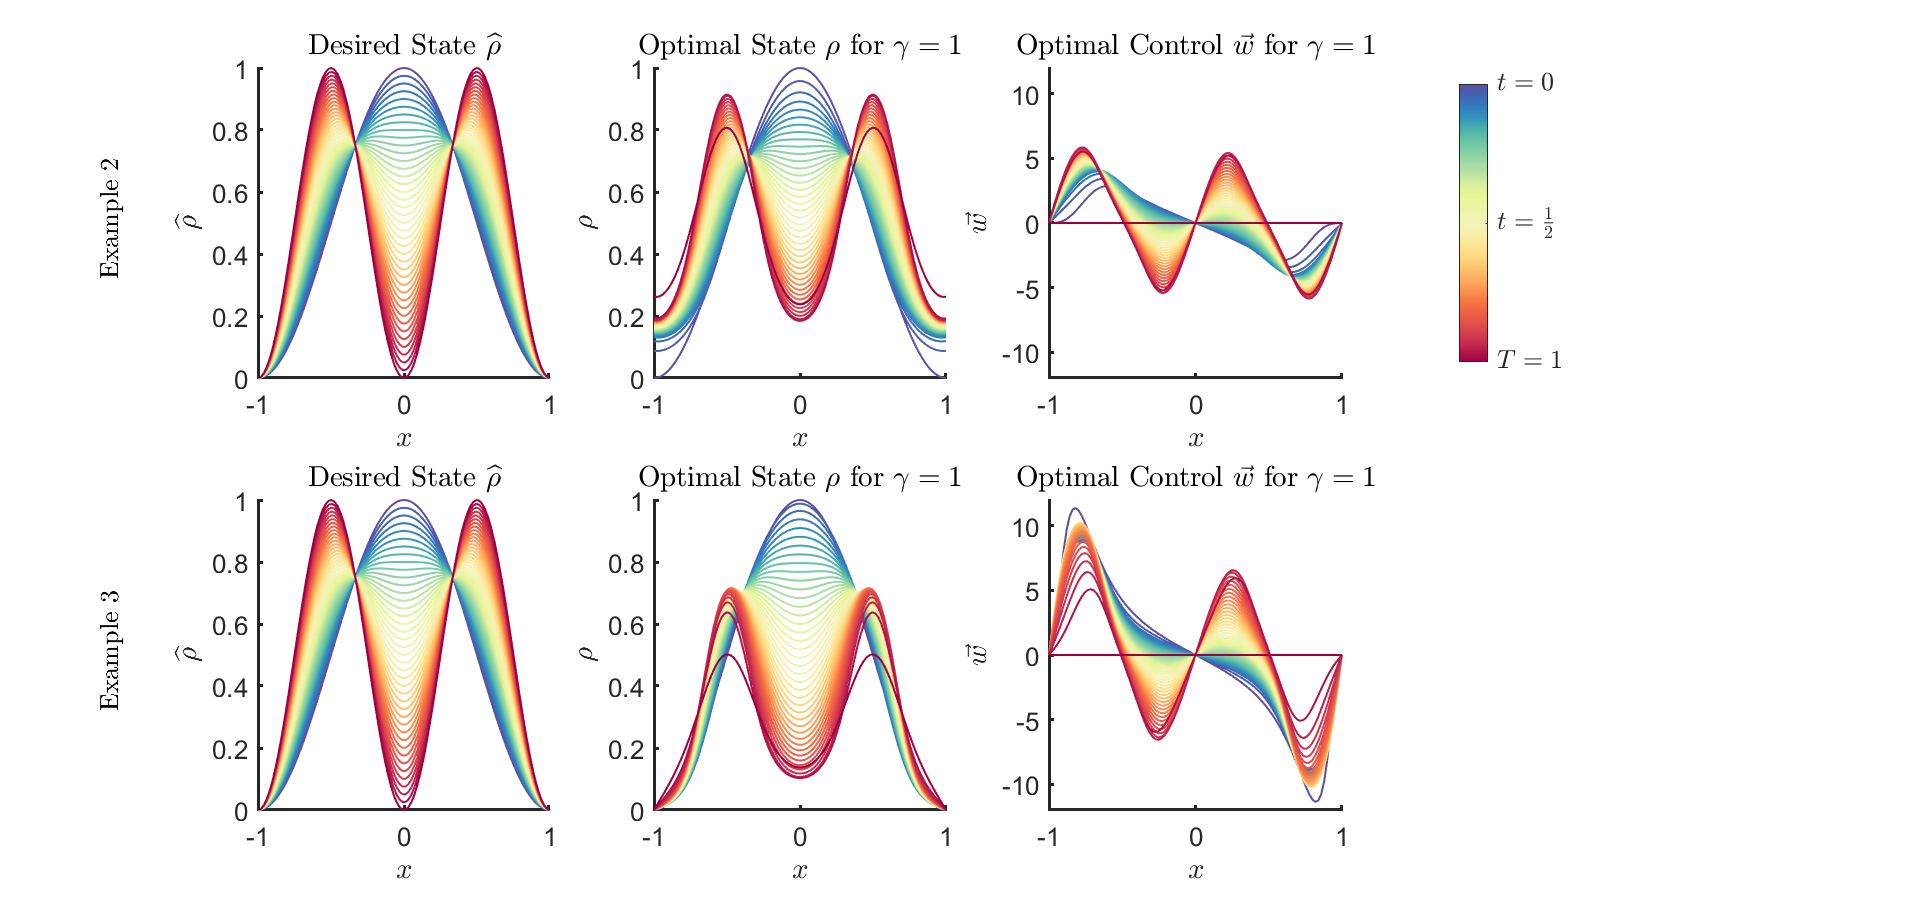
\includegraphics[scale=0.05]{Figure3.png}
	\caption{Example 2/ Example 3, desired state $\widehat \rho$, optimal state $\rho$ and corresponding optimal control $\vec{w}$, $\beta = 10^{-3}$, $\gamma = 1$.}
	\label{Ex22DN1}
\end{figure}

\begin{table}
\begin{tabular}{ | c | c || c | c | c | c ||}
\hline
\multicolumn{2}{|c||}{}& $\beta = 10^{-3}$ & $\beta = 10^{-1}$ & $\beta = 10^{1}$ & $\beta = 10^{3}$  \\
\hline
\hline
 & $\mathcal{J}_{uc}$ & $\numprint{0.0536}$ & $\numprint{0.0536}$ & $\numprint{0.0536}$ & $\numprint{0.0536}$ \\
$\kappa= \numprint{-1}$  & $\mathcal{J}_c$ & $\numprint{0.0096}$ & $\numprint{0.0492}$ & $\numprint{0.0535}$ & $\numprint{0.0536}$ \\
& \texttt{Iter} & $\numprint{715}$ & $\numprint{767}$ & $\numprint{367}$ & $\numprint{1}$ \\
\hline
 & $\mathcal{J}_{uc}$ & $\numprint{0.0669}$ & $\numprint{0.0669}$ & $\numprint{0.0669}$ & $\numprint{0.0669}$ \\
$\kappa= \numprint{0}$  & $\mathcal{J}_c$ & $\numprint{0.0109}$ & $\numprint{0.0603}$ & $\numprint{0.0668}$ & $\numprint{0.0669}$ \\
& \texttt{Iter} & $\numprint{714}$ & $\numprint{770}$ & $\numprint{390}$ & $\numprint{1}$ \\
\hline
 & $\mathcal{J}_{uc}$ & $\numprint{0.0839}$ & $\numprint{0.0839}$ & $\numprint{0.0839}$ & $\numprint{0.0839}$ \\
$\kappa= \numprint{1}$  & $\mathcal{J}_c$ & $\numprint{0.0125}$ & $\numprint{0.0748}$ & $\numprint{0.0838}$ & $\numprint{0.0839}$ \\
& \texttt{Iter} & $\numprint{713}$ & $\numprint{773}$ & $\numprint{403}$ & $\numprint{1}$ \\
\hline
\end{tabular}
\caption{Example 2: Cost when $\vec{w}=\vec{0}$, optimal control cost, and iterations required, for a range of $\kappa$, $\beta$.}
\label{TabS5:Prob2}
\end{table} %\label{TabS5:Prob2a}


\subsubsection{Dirichlet boundary conditions, Example 3} 
The inputs for this example are:
\begin{align*}
&\widehat \rho = \bigg(\frac{1}{2}\cos(\pi y) + \frac{1}{2}\bigg)(1-t) + t\bigg(-\frac{1}{2}\cos(2 \pi y) + \frac{1}{2}\bigg),\\
&\rho_{0} = \frac{1}{2}\cos(\pi y) + \frac{1}{2},\ \
\adj_{T} = 0,\ \
\vec{w} = \vec{0},\ \
f =0,\ \
V_{ext} =0.
\end{align*}
Table \ref{TabS5:Prob3} presents the results for this example, for a range of $\beta$ values and different interaction strengths. The observations are in line with those in Example 1 and 2. In particular, $ \widehat \rho$ and $\rho_0$ coincide with those of the problem with Neumann boundary conditions in Example 2. A comparison between the two examples is illustrated in Figure \ref{Ex22DN1}. Both the optimal state $\rho$ and the optimal control are qualitatively different when considering Dirichlet boundary conditions over Neumann conditions. The numerical result for this example was achieved with $N=40$ and $n = 30$, rather than with $N=30$ and $n=20$. This indicates that the Dirichlet boundary conditions are harder to apply in this problem, due to the steep shape of the desired state. This steepness is somewhat less impactful in Example 2, where the desired state is not closely matched by the optimal state at the boundaries. In Example 3, while the optimal state matches the desired state perfectly at the boundary, the peaks of the desired state are matched less closely. In Figure \ref{Ex22DN1}, this can be confirmed by considering the control plots. The optimal control for Example 3 is larger than for Example 2, specifically between the boundaries of the domain and the peaks of the desired state, indicating difficulties in this region.
\begin{table}
\begin{tabular}{ ||c|| c | c | c | c | c ||}
\hline
& & $\beta = 10^{-3}$ & $\beta = 10^{-1}$ & $\beta = 10^{1}$ & $\beta = 10^{3}$  \\
\hline
 & $J_{uc}$ & $\numprint{1.4165e-1}$ & $\numprint{1.4165e-1}$ & $\numprint{1.4165e-1}$ & $\numprint{1.4165e-1}$ \\
$\gamma= \numprint{-1}$  & $J_c$ & $\numprint{3.5594e-2}$ & $\numprint{1.3270e-1}$ & $\numprint{1.4155e-1}$ & $\numprint{1.4165e-1}$ \\
& $Iter.$ & $\numprint{944}$ & $\numprint{816}$ & $\numprint{437}$ & $\numprint{1}$ \\
\hline
 & $J_{uc}$ & $\numprint{1.5452e-1}$ & $\numprint{1.5452e-1}$ & $\numprint{1.5452e-1}$ & $\numprint{1.5452e-1}$ \\
$\gamma= \numprint{0}$  & $J_c$ & $\numprint{3.8023e-2}$ & $\numprint{1.4549e-1}$ & $\numprint{1.5442e-1}$ & $\numprint{1.5452e-1}$ \\
& $Iter.$ & $\numprint{940}$ & $\numprint{825}$ & $\numprint{440}$ & $\numprint{1}$ \\
\hline
 & $J_{uc}$ & $\numprint{1.6610e-1}$ & $\numprint{1.6610e-1}$ & $\numprint{1.6610e-1}$ & $\numprint{1.6610e-1}$ \\
$\gamma= \numprint{1}$  & $J_c$ & $\numprint{4.1143e-2}$ & $\numprint{1.5751e-1}$ & $\numprint{1.6601e-1}$ & $\numprint{1.6610e-1}$ \\
& $Iter.$ & $\numprint{932}$ & $\numprint{827}$ & $\numprint{440}$ & $\numprint{1}$ \\
\hline
\end{tabular}
\caption{Problem 3 ($n = 30,N = 40$)}
\label{TabS5:Prob3}
\end{table} %\label{TabS5:Prob3}


%\subsubsection{Neumann boundary conditions, Symmetric Example 1}
%Consider the following symmetric setup:
%\begin{align*}
%\widehat \rho &= \frac{1}{2}(1-t) + t\frac{1}{4}(\cos(\pi y)+2),\\
%\rho_{0} &= \frac{1}{2},\  \ q_{T} = 0, \ \ \vec{w} = \vec{0}, \ \  f =0, \ \ V_{ext} =0.
%\end{align*}
%Table \ref{TabNFlowAddEx1} summarizes the results for this example.The attractive interaction term causes $\rho$ to move towards the centre of the domain. Since $\widehat \rho$ is also centred in the domain, $J_{uc}$ is small for $\gamma =-1$ in comparison to the problems with $\gamma =0$ and $\gamma =1$. This example illustrates that the particle interaction term can have a significant impact on the optimization problem considered. 
%
%
%
%
%\subsubsection{Neumann boundary conditions, Symmetric Example 2}
%Consider the following symmetric setup, which is the opposite of the first symmetric example:
%\begin{align*}
%\widehat \rho &= \frac{1}{2}(1-t) + t\frac{1}{4}(-\cos(\pi y)+2),\\
%\rho_{0} &= \frac{1}{2},\ \
%q_{T} = 0,\ \
%\vec{w} = \vec{0},\ \
%f =0,\ \
%V_{ext} =0.
%\end{align*}
%This example can be compared to the Symmetric Example 1. Here, the desired state is having $\rho$ clustered at both boundaries, which is similar to the effect of the repulsive interaction term $\gamma = 1$. Therefore, for this choice of interaction term, the value of the cost functional $J_{uc}$ is smaller than the one for $\gamma = 0$ and $\gamma = -1$. This is the opposite to the observation made in the Symmetric Example 1, which is to be expected, given the two choices of desired state.


\subsection{Linear control problems with an additional nonlocal integral term}
In this section, examples of solving Problem \eqref{AdvDiff_Linear} with both 'no-flux type' boundary conditions \eqref{NoFlux_Linear} and Dirichlet boundary conditions \eqref{Dirichlet}.
\subsubsection{Dirichlet boundary conditions, Example 4}
The inputs for this example are:
\begin{align*}
&\widehat \rho = (1 - t)\bigg(\frac{1}{2}\cos(\pi y) + \frac{1}{2}\bigg)  + t\bigg(-\frac{1}{2}\cos(\pi y) + \frac{1}{2}\bigg),\\
&\rho_{0} = \frac{1}{2}\cos(\pi y) + \frac{1}{2},\ \
\adj_{T} = 0,\ \
{w} = 0,\ \
f =0, \ \
V_{ext} =\frac{1}{2}\left((x + 0.3)^2 - 0.2\right)\left((x-0.4)^2 - 0.3\right).
\end{align*}
In Table \ref{TabS5:Prob4} the results for Example 4 for a range of parameter values can be found. The results are qualitatively similar to the previous examples, but the control is applied linearly in this example. Note that here $\lambda = 0.005$, since $V_{{ext}}$ causes the numerical computations to be more challenging.
\begin{table}
\begin{tabular}{ | c | c || c | c | c | c ||}
\hline
\multicolumn{2}{|c||}{}& $\beta = 10^{-3}$ & $\beta = 10^{-1}$ & $\beta = 10^{1}$ & $\beta = 10^{3}$  \\
\hline
\hline
 & $\mathcal{J}_{uc}$ & $\numprint{0.1394}$ & $\numprint{0.1394}$ & $\numprint{0.1394}$ & $\numprint{0.1394}$ \\
$\kappa= \numprint{-1}$  & $\mathcal{J}_c$ & $\numprint{0.0183}$ & $\numprint{0.0862}$ & $\numprint{0.1384}$ & $\numprint{0.1394}$ \\
& \texttt{Iter} & $\numprint{1575}$ & $\numprint{1486}$ & $\numprint{1026}$ & $\numprint{117}$ \\
\hline
 & $\mathcal{J}_{uc}$ & $\numprint{0.1526}$ & $\numprint{0.1526}$ & $\numprint{0.1526}$ & $\numprint{0.1526}$ \\
$\kappa= \numprint{0}$  & $\mathcal{J}_c$ & $\numprint{0.0183}$ & $\numprint{0.0983}$ & $\numprint{0.1516}$ & $\numprint{0.1526}$ \\
& \texttt{Iter} & $\numprint{1582}$ & $\numprint{1474}$ & $\numprint{1023}$ & $\numprint{113}$ \\
\hline
 & $\mathcal{J}_{uc}$ & $\numprint{0.1645}$ & $\numprint{0.1645}$ & $\numprint{0.1645}$ & $\numprint{0.1645}$ \\
$\kappa= \numprint{1}$  & $\mathcal{J}_c$ & $\numprint{0.0189}$ & $\numprint{0.1103}$ & $\numprint{0.1635}$ & $\numprint{0.1645}$ \\
& \texttt{Iter} & $\numprint{1589}$ & $\numprint{1465}$ & $\numprint{1022}$ & $\numprint{112}$ \\
\hline
\end{tabular}
\caption{Example 4: Uncontrolled cost $\mathcal{J}_{uc}$, optimal cost $\mathcal{J}_{c}$, and number of iterations, for a range of $\kappa$ and $\beta$ values.}
\label{TabS5:Prob4}
\end{table} %\label{TabS5:Prob4}




\subsubsection{Neumann boundary conditions, Example 5}
The inputs for this example are:
\begin{align*}
&\widehat \rho = \frac{1}{2}(1-t) + t\frac{1}{2}(-\cos(\pi y) + 1),\\
&\rho_{0} = \frac{1}{2},\ \
\adj_{T} = 0,\ \
{w} = 0,\ \
f =0,\ \
V_{ext} =0.
\end{align*}
Table \ref{TabS5:Prob5} shows the results for Example 5. Note that for this example, when $\beta = 10^{-3}$, the mixing parameter $\lambda$ had to be set to $0.001$, to guarantee stable convergence of the method (why? explanation needed?).
Again, the only qualitative difference to interpreting the results is that the control is applied linearly.
\begin{table}
\begin{tabular}{ ||c|| c | c | c | c | c ||}
\hline
& & $\beta = 10^{-3}$ & $\beta = 10^{-1}$ & $\beta = 10^{1}$ & $\beta = 10^{3}$  \\
\hline
 & $J_{uc}$ & $\numprint{6.0640e-2}$ & $\numprint{6.0640e-2}$ & $\numprint{6.0640e-2}$ & $\numprint{6.0640e-2}$ \\
$\gamma= \numprint{-1}$  & $J_c$ & $\numprint{6.0180e-3}$ & $\numprint{5.5365e-2}$ & $\numprint{6.0592e-2}$ & $\numprint{6.0640e-2}$ \\
& $Iter.$ & $\numprint{7320}$ & $\numprint{7712}$ & $\numprint{3888}$ & $\numprint{1}$ \\
\hline
 & $J_{uc}$ & $\numprint{4.1667e-2}$ & $\numprint{4.1667e-2}$ & $\numprint{4.1667e-2}$ & $\numprint{4.1667e-2}$ \\
$\gamma= \numprint{0}$  & $J_c$ & $\numprint{4.5414e-3}$ & $\numprint{3.8334e-2}$ & $\numprint{4.1632e-2}$ & $\numprint{4.1667e-2}$ \\
& $Iter.$ & $\numprint{7271}$ & $\numprint{7614}$ & $\numprint{3643}$ & $\numprint{1}$ \\
\hline
 & $J_{uc}$ & $\numprint{2.8551e-2}$ & $\numprint{2.8551e-2}$ & $\numprint{2.8551e-2}$ & $\numprint{2.8551e-2}$ \\
$\gamma= \numprint{1}$  & $J_c$ & $\numprint{3.5942e-3}$ & $\numprint{2.6480e-2}$ & $\numprint{2.8529e-2}$ & $\numprint{2.8551e-2}$ \\
& $Iter.$ & $\numprint{7249}$ & $\numprint{7482}$ & $\numprint{3410}$ & $\numprint{1}$ \\
\hline
\end{tabular}
\caption{Problem 5}
\label{TabS5:Prob5}
\end{table} %\label{TabS5:Prob5}


\subsection{Nonlinear control problems with an additional nonlocal integral term in 2D}
In this section, two-dimensional examples are considered, to illustrate the fact that the application of the method differs very little from the one dimensional setting. The main difference is that in nonlinear control problems the control is a two-dimensional vector field. Furthermore, the number of spatial points increases from $N$ to $N_1\times N_2$, which makes computations much more costly. Compensating for this increased cost is one of the motivations to develop fast optimization solvers, such as the fixed point method introduced in Section \ref{sec:Method_Solver}.
\subsubsection{Neumann boundary conditions, Example 1}	
We have the following set up:
\begin{align*}
&\widehat \rho = \frac{1}{4}(1-t) + t\bigg(\frac{1}{4}\sin \bigg(\frac{\pi}{2}(x_1 - 2)\bigg)\sin \bigg(\frac{\pi}{2}(x_2 - 2)\bigg) + \frac{1}{4}\bigg),\\
&\rho_0 = \frac{1}{4},\ \
q_{T} = 0,\ \
\vec{w} = \vec{0},\ \
f =0,\ \
V_{ext} =0.
\end{align*}
This example is the two dimensional version of Example 1 in Section \ref{sec:Examples1d}. The results for this example are displayed in Table \ref{TabS5:Prob12D}. In Figures \ref{rhoHat2dEx2} it can be observed that as in Example 1 in Section \ref{sec:Examples1d}, the uncontrolled state forms a cluster in the centre of the domain, due to the attractive interactions. Figure \ref{rhoOpt2dEx2} shows the optimal state and control for different time points, for $\beta = 10^{-3}$ and $\gamma = -1$. Here, the control through a vector field illustrates why nonlinear control is called 'flow control'. 

\begin{table}
\begin{tabular}{ ||c|| c | c | c | c | c ||}
\hline
& & $\beta = 10^{-3}$ & $\beta = 10^{-1}$ & $\beta = 10^{1}$ & $\beta = 10^{3}$  \\
\hline
 & $\mathcal J_{\vec w = \vec 0}$ & $0.0113$ & $0.0113$ & $0.0113$ & $0.0113$ \\
$\kappa= -1$  & $\mathcal J_{Opt}$ & $0.0013$ & $0.0104$ & $0.0113$ & $0.0113$ \\
& $\text{Iterations}$ & $676$ & $700$ & $290$ & $1$ \\
\hline
\end{tabular}
\caption{Results for the test problem, with different $\beta$}
\label{TabS5:Prob12D}
\end{table} % \label{TabS5:Prob12D}

\begin{figure}[h]
	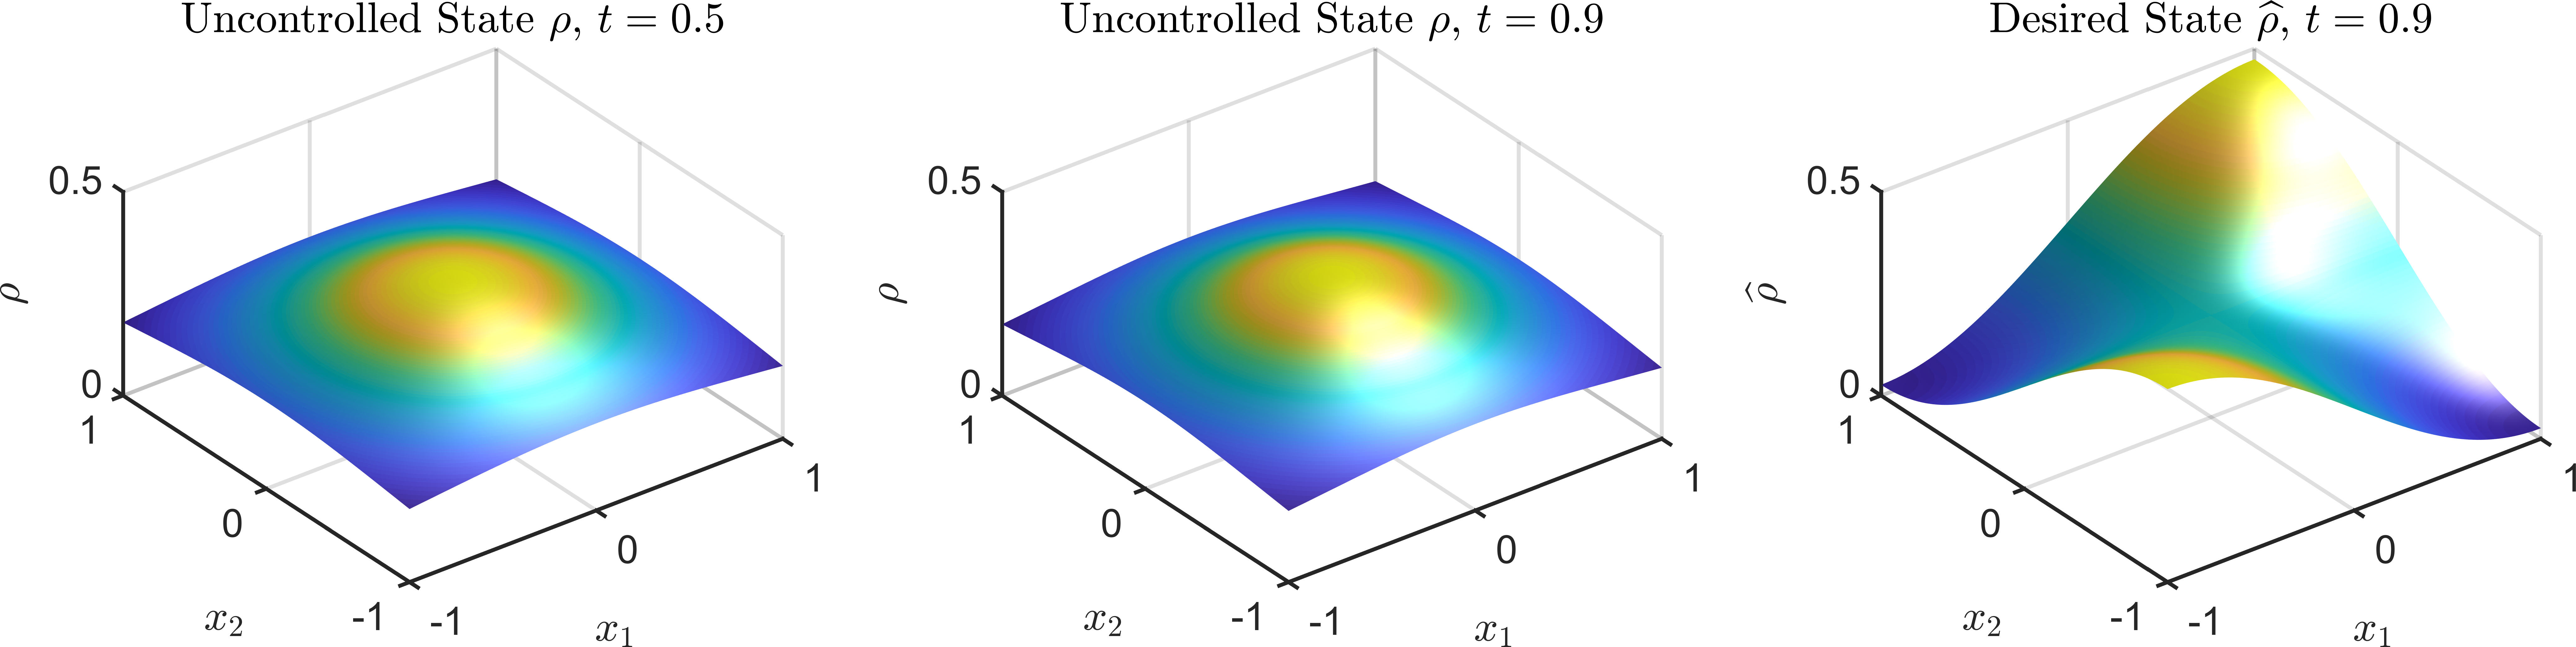
\includegraphics[scale=0.05]{Figure12D.png}
	\caption{2D Example 1, uncontrolled $\rho$ and $\widehat \rho$, $\beta = 10^{-3}$, $\gamma = -1$.}
	\label{rhoHat2dEx2}
\end{figure}
\begin{figure}[h]
	\includegraphics[scale=0.06]{Figure22D.png}
	\caption{2D Example 1, controlled $\rho$ and optimal control $\vec{w}$, $\beta = 10^{-3}$, $\gamma = -1$.}
	\label{rhoOpt2dEx2}
\end{figure}


\subsubsection{Neumann boundary conditions, Example 2}	
Here, we have:
\begin{align*}
&\widehat \rho = \frac{1}{4}(1-t) + t\frac{1}{0.9921}e^{-3((y_1+0.2)^2 + (y_2+0.2)^2))},\\
&\rho_0 = \frac{1}{4},\ \
q_{T} = 0,\ \
\vec{w} = \vec{0},\ \
f =0,\\
&V_{ext} =\left((x_1 + 0.3)^2 - 1\right)\left((x_1-0.4)^2 - 0.5\right)
\left((x_2 + 0.3)^2 - 1\right)\left((x_2-0.4)^2 - 0.5\right).
\end{align*}
The numerical results for this example are displayed in Table \ref{TabS5:Prob22D}. In figures \ref{rhoHat2dEx4} and \ref{rhoOpt2dEx4} the results are illustrated for $\beta = 10^{-3}$ and $\gamma = -1$. It can be observed very clearly that the control is driving the particle distribution to the desired state. It is noticeable that the control does not act uniformly around the peak of the desired state, but also acts strongly in the area between the location of the desired peak and the point $(-1,1)$. This is due to the external potential being steep in this area and more control is needed to reach the desired state than in other parts of the domain.

\begin{table}
\begin{tabular}{ | c | c || c | c | c | c ||}
\hline
\multicolumn{2}{|c||}{}& $\beta = 10^{-3}$ & $\beta = 10^{-1}$ & $\beta = 10^{1}$ & $\beta = 10^{3}$  \\
\hline
\hline
 & $\mathcal{J}_{uc}$ & $\numprint{0.0378}$ & $\numprint{0.0378}$ & $\numprint{0.0378}$ & $\numprint{0.0378}$ \\
$\kappa= \numprint{-1}$  & $\mathcal{J}_c$ & $\numprint{0.0017}$ & $\numprint{0.0312}$ & $\numprint{0.0377}$ & $\numprint{0.0378}$ \\
& \texttt{Iter} & $\numprint{691}$ & $\numprint{736}$ & $\numprint{347}$ & $\numprint{1}$ \\
\hline
 & $\mathcal{J}_{uc}$ & $\numprint{0.0478}$ & $\numprint{0.0478}$ & $\numprint{0.0478}$ & $\numprint{0.0478}$ \\
$\kappa= \numprint{0}$  & $\mathcal{J}_c$ & $\numprint{0.0064}$ & $\numprint{0.0450}$ & $\numprint{0.0478}$ & $\numprint{0.0478}$ \\
& \texttt{Iter} & $\numprint{718}$ & $\numprint{784}$ & $\numprint{343}$ & $\numprint{1}$ \\
\hline
 & $\mathcal{J}_{uc}$ & $\numprint{0.0526}$ & $\numprint{0.0526}$ & $\numprint{0.0526}$ & $\numprint{0.0526}$ \\
$\kappa= \numprint{1}$  & $\mathcal{J}_c$ & $\numprint{0.0137}$ & $\numprint{0.0514}$ & $\numprint{0.0526}$ & $\numprint{0.0526}$ \\
& \texttt{Iter} & $\numprint{735}$ & $\numprint{790}$ & $\numprint{338}$ & $\numprint{1}$ \\
\hline
\end{tabular}
\caption{2D Ex. 2: Uncontrolled cost $\mathcal{J}_{uc}$, optimal cost $\mathcal{J}_{c}$, and number of iterations, for a range of $\kappa$ and $\beta$ values.}
\label{TabS5:Prob22D}
\end{table} %\label{TabS5:Prob22D}

\begin{figure}[h]
	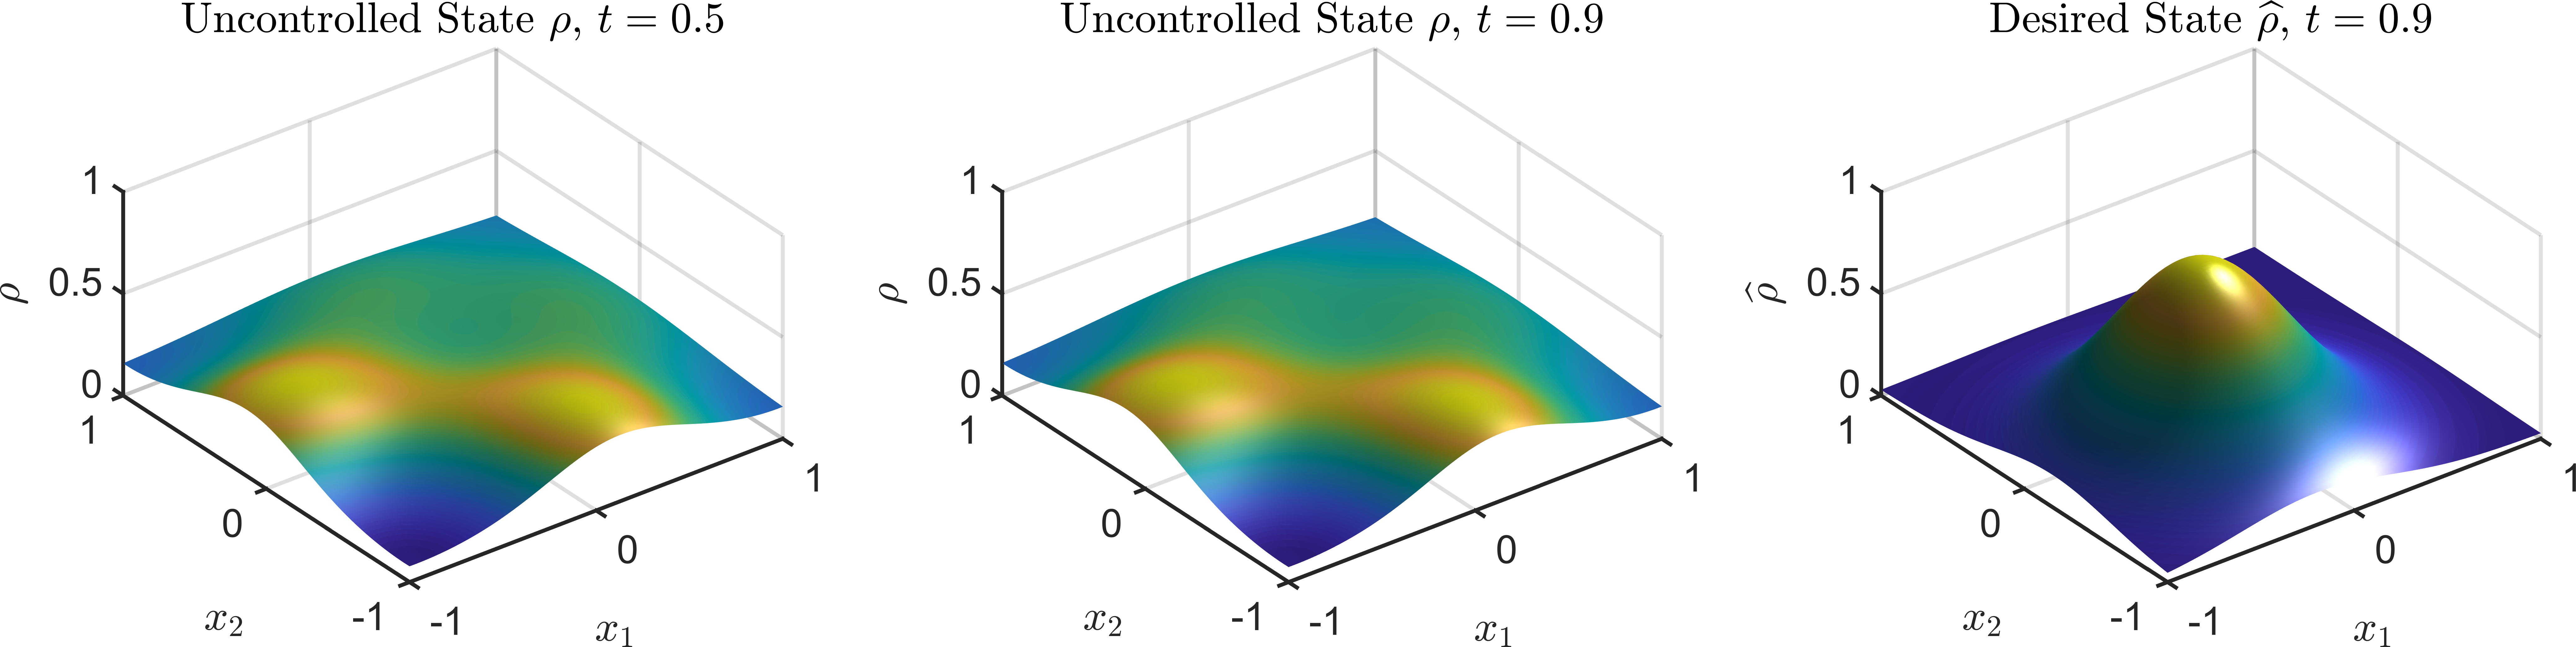
\includegraphics[scale=0.05]{Figure32D.png}
	\caption{2D Example 2: Uncontrolled $\rho$ and desired state $\widehat \rho$,  with $\beta = 10^{-3}$ and $\kappa = -1$. }
	\label{rhoHat2dEx4}
\end{figure}
\begin{figure}[h]
	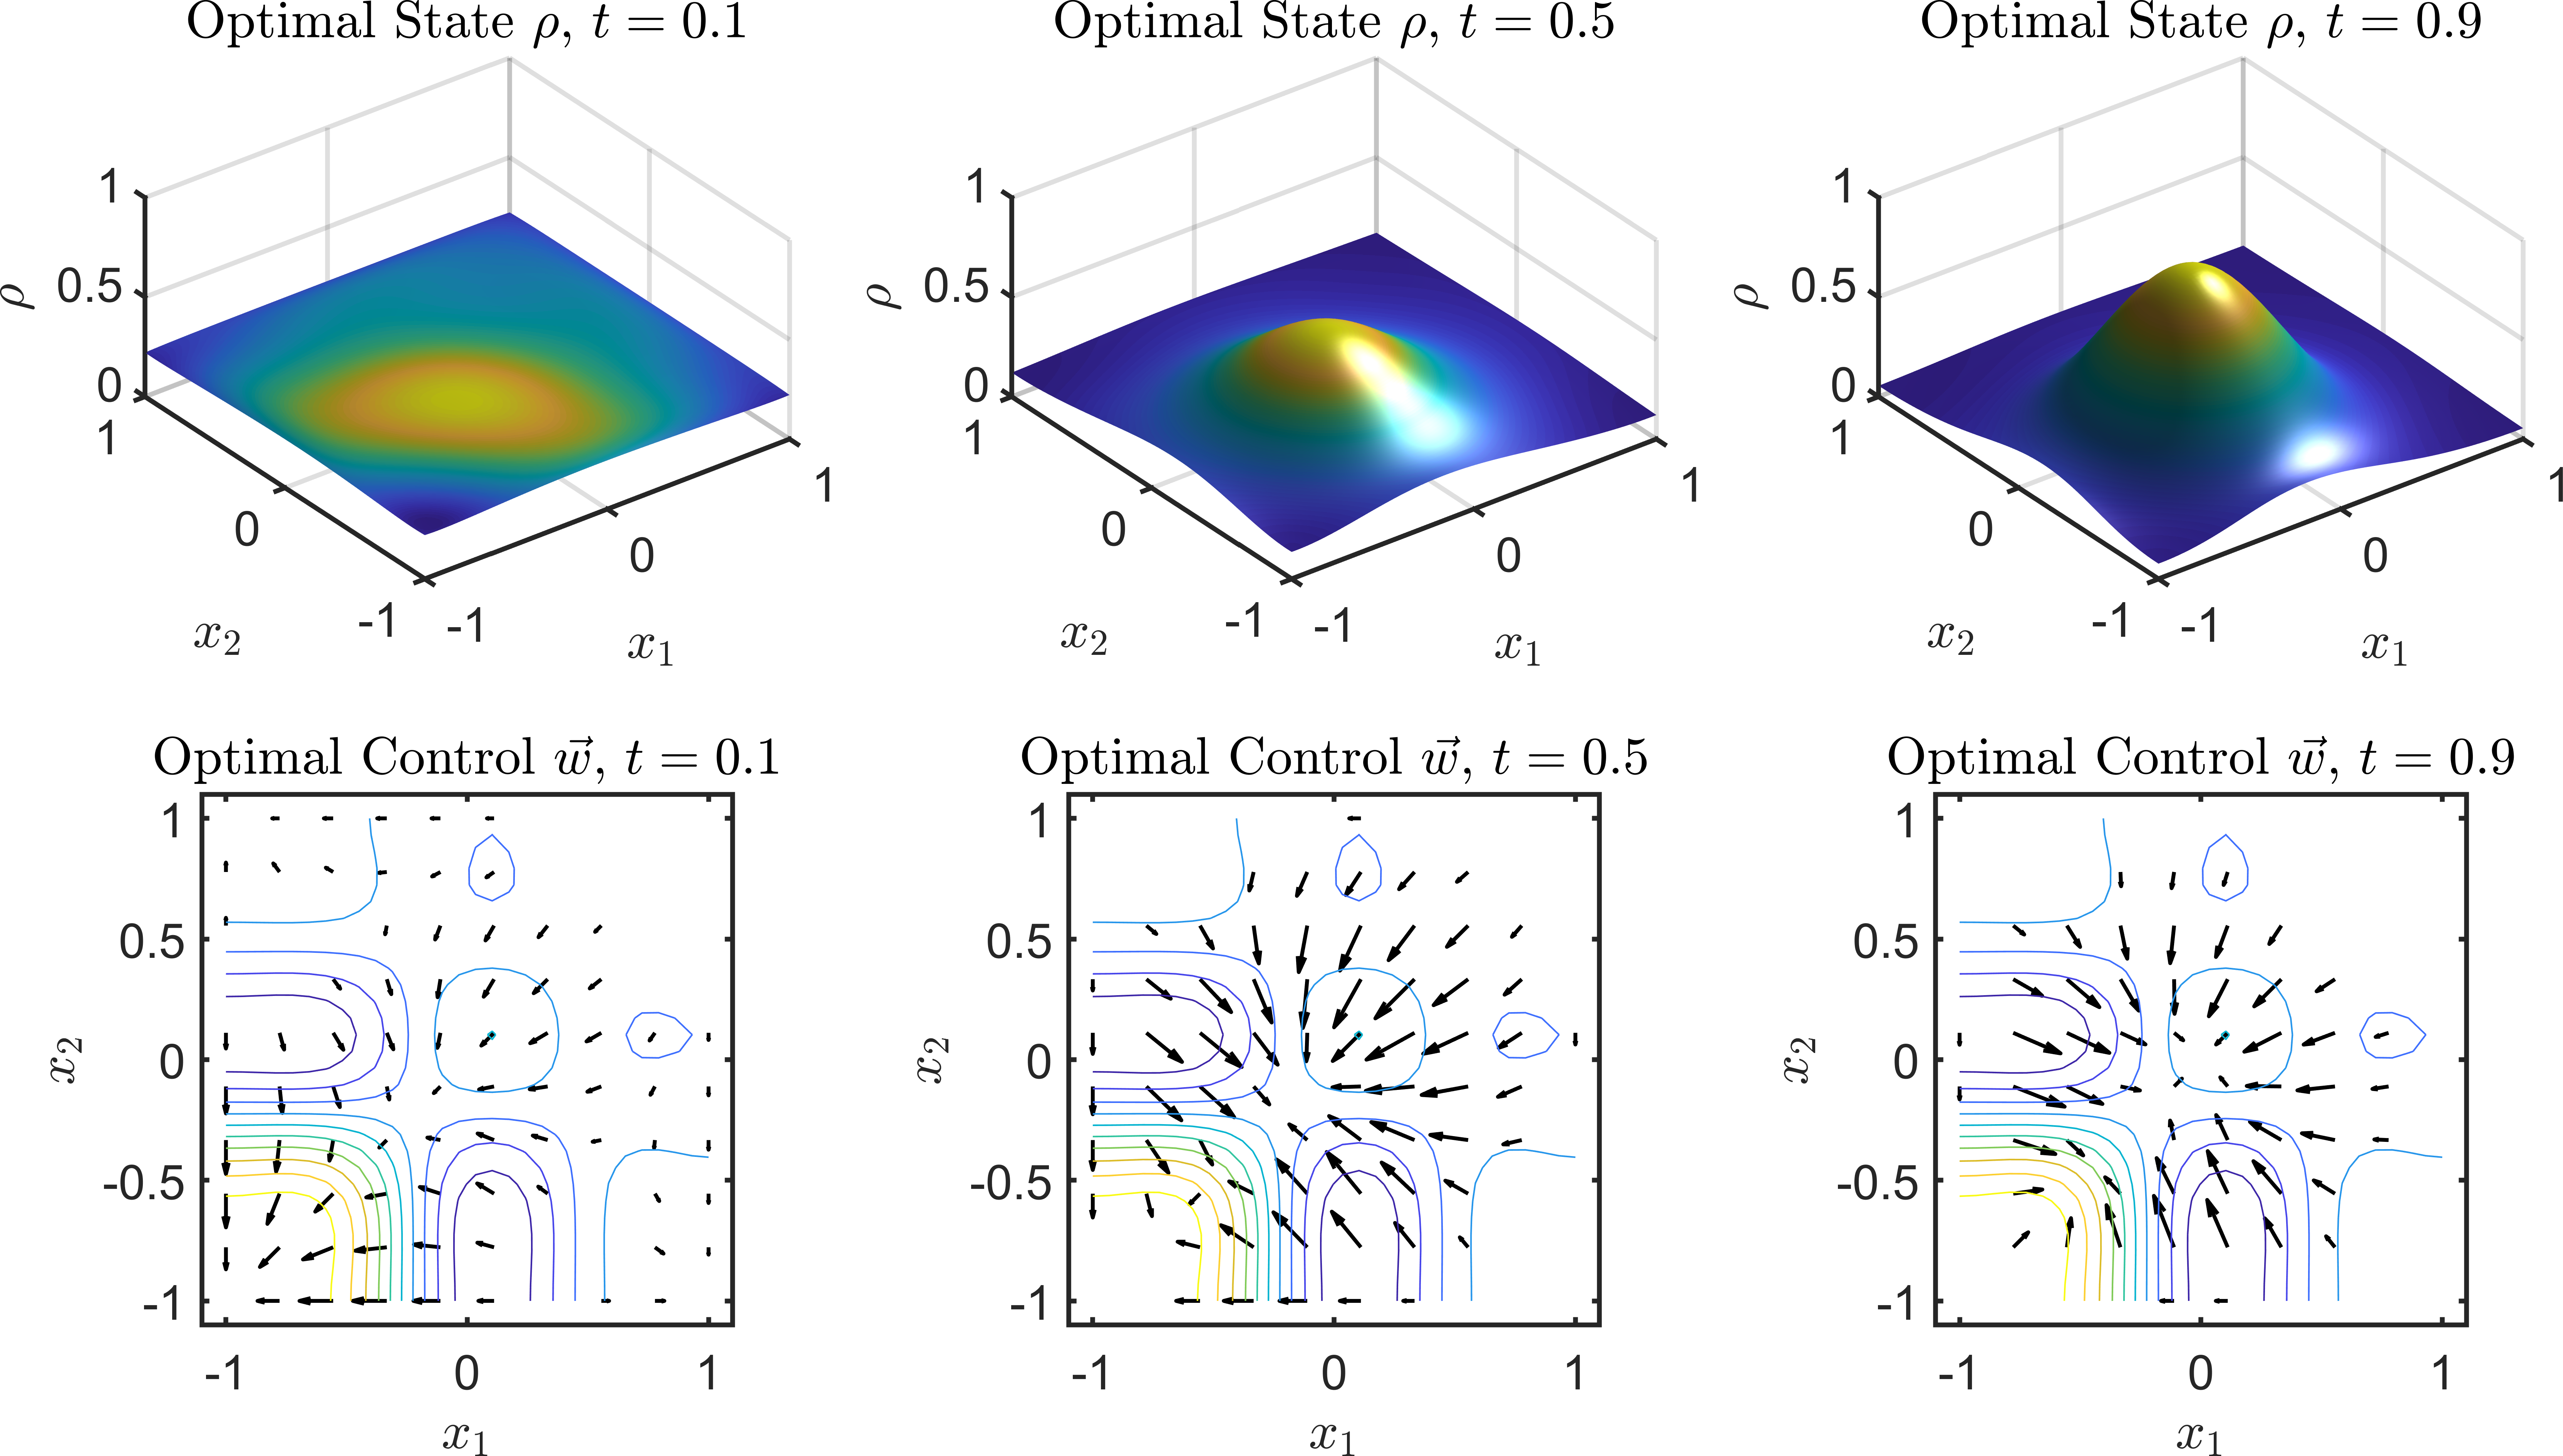
\includegraphics[scale=0.06]{Figure42D.png}
	\caption{2D Example 2: Optimal state $\rho$ and optimal control $\vec{w}$, with $\beta = 10^{-3}$ and $\kappa = -1$. A contour plot of the external potential $V^{\text{ext}}$ is superimposed on the control plots for reference.} 
	\label{rhoOpt2dEx4}
\end{figure}









\section{Conclusion}
+ outlook!


\pagebreak	
\bibliography{GeneralBib}
\bibliographystyle{unsrt}

\pagebreak
\appendix

\section{Other thoughts - things to incorporate above}
- mass correction if mass is to be one\\


\section{Useful Resources to go back to}
'A practical guide to pseudospectral methods', Bengt Fornberg\\
van kampen stochastic processes in physics and chemistry
\end{document}